%\section{\centering Experimental Setup}
\chapter{Radiation Tolerance of 65 nm CMOS Transistors}
%\chapter*{\centering Experimental Setup}
\label{ch:RadStudies}

The need for extremely radiation tolerant electronics, especially in the era of High Luminosity running at the LHC (HL-LHC), is a major issue confronting high energy physics. The HL-LHC will begin running in 2025 and the expected peak luminosity is $5\times10^{34}\; \mathrm{cm}^{-2}\mathrm{s}^{-1}$. At this luminosity, the particle flux near the collision vertex will be extremely high and the electronics in the pixel detector will need to be able to operate while accumulating a total ionizing dose of about 1 Grad. 

To lower the material density and power dissipation in the pixel detector, the plan for the HL-LHC readout chips in the pixel detector at CMS is to upgrade from the current 130 nm complementary metal-oxide-semiconductor (CMOS) technology to 65 nm CMOS technology. Previous studies~\cite{CMOSXrayRadiation} showed that the properties of 65 nm CMOS technology did not dramatically change after being exposed to a total dose of 200 Mrad. However, these studies were conducted at room temperature and the pixel detector will be operated at $-20^{\circ}\mathrm{C}$ to limit the leakage current in the silicon strip trackers. At a lower temperature, the CMOS devices will not anneal as much and the radiation damage might be greater than had been observed in room temperature exposures. Thus, it is important to characterize the response of 65 nm CMOS technology to large radiation doses while operating at $-20^{\circ}\mathrm{C}$.

This chapter summarizes an experiment~\cite{CMOSRadiation} that characterized the response of 65 nm CMOS transistors to a cumulative radiation dose of 1 Grad while being held below $-20^{\circ}\mathrm{C}$.

\section{Radiation Damage Mechanisms}

Two types of radiation damage can occur when energetic particles pass through a semiconductor device and either electron-hole pairs (ionization damage) are created or silicon atoms are displaced from their lattice sites (displacement damage). This chapter will focus on ionization damage. 

Ionization damage occurs in the insulating layers of the device, usually $\ce{SiO_{2}}$, when the electrons and holes drift to different locations where they are trapped and cause unwanted electromagnetic fields within the device. There are two locations of insulating layers within current semiconductors: the gate oxide and the shallow trench isolation (STI) oxide. A layout of a CMOS transistor can be seen in Figure~\ref{fig:CMOS_Layout}\cite{CMOSLayout}.

\begin{figure}[htbp]
\begin{center}
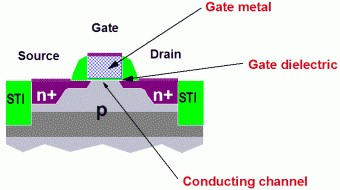
\includegraphics[width=4 in]{RadiationStudies/CMOS_Layout_2.jpg}
\end{center}
\caption{The cross section view of an n-channel transistor. The transistor is built on a p-type substrate with n-type implants as the source and drain. An inversion layer is formed in the conducting channel when a positive voltage is applied to the gate. The gate dielectric (gate oxide) and shallow trench isolation (STI) oxide are the green regions\cite{CMOSLayout}.}
\label{fig:CMOS_Layout}
\end{figure}

Gate oxide separates the gate terminal from the conductive channel that connects the source and drain and serves as a dielectric layer so that the gate can sustain a high electric field. When electron-hole pairs are created in the gate oxide the electrons are swept out of the oxide by the positive voltage applied on the gate terminal while holes move in the opposite direction toward the Si/$\ce{SiO_{2}}$ interface. Two separate mechanisms can then occur~\cite{TIDEffects}: 
\begin{itemize}
\item \textbf{Deep Hole Trapping:}  There is a transition region from $\ce{SiO_{2}}$ to Si where the oxidation is not complete and there are oxygen vacancies. These vacancies cause weak Si-Si bonds, where each Si atom is also bonded to three oxygen atoms, that are broken by holes which then remain trapped there. The holes accumulate at the interface causing a buildup of positive charge.
\item \textbf{Radiation-Induced Traps:} At the Si/$\ce{SiO_{2}}$ interface there are tri-valent Si atoms that have been passivated by H atoms. Radiation-induced holes free protons from the oxide and the protons then travel to the Si/$\ce{SiO_{2}}$ interface. At the interface the proton breaks the Si-H bond to form $\ce{H_{2}}$ and a trivalent Si atom that is left with an unpassivated dangling bond that is an electrically active defect.
\end{itemize}
These effects cause the voltage seen by the conductive channel to differ from the actual voltage applied at the gate terminal and thus, the transistor will turn on at a different voltage than it was designed to. These mechanisms are extremely dependent on the thickness of the gate oxide and more deep hole and radiation-induced traps will build up the thicker the gate oxide is. 

STI oxide is implanted in the silicon between adjacent semiconductors to prevent leakage current. The same mechanisms that occur in the gate oxide also occur in the STI oxide, however they effect the transistor functionality differently. When charge builds up in the STI oxide, a conductive channel is opened between the source and drain of the transistor and leakage current can flow even when the transistor is turned off. This is illistrated in Figure~\ref{fig:LeakageCurrent}\cite{LeakageCurrent}. 

The radiation induced charge that is trapped in the STI also prevents channel inversion near the STI and reduces the conductive channel width. This is referred to as Radiation Induced Narrow Channel Effect (RINCE)\cite{RINCE} and is more evident in narrow channel devices. A narrower conductive channel allows less current to flow from the source to drain and thus, the maximum drain to source current that can be achieved is decreased.

\begin{figure}[htbp]
\begin{center}
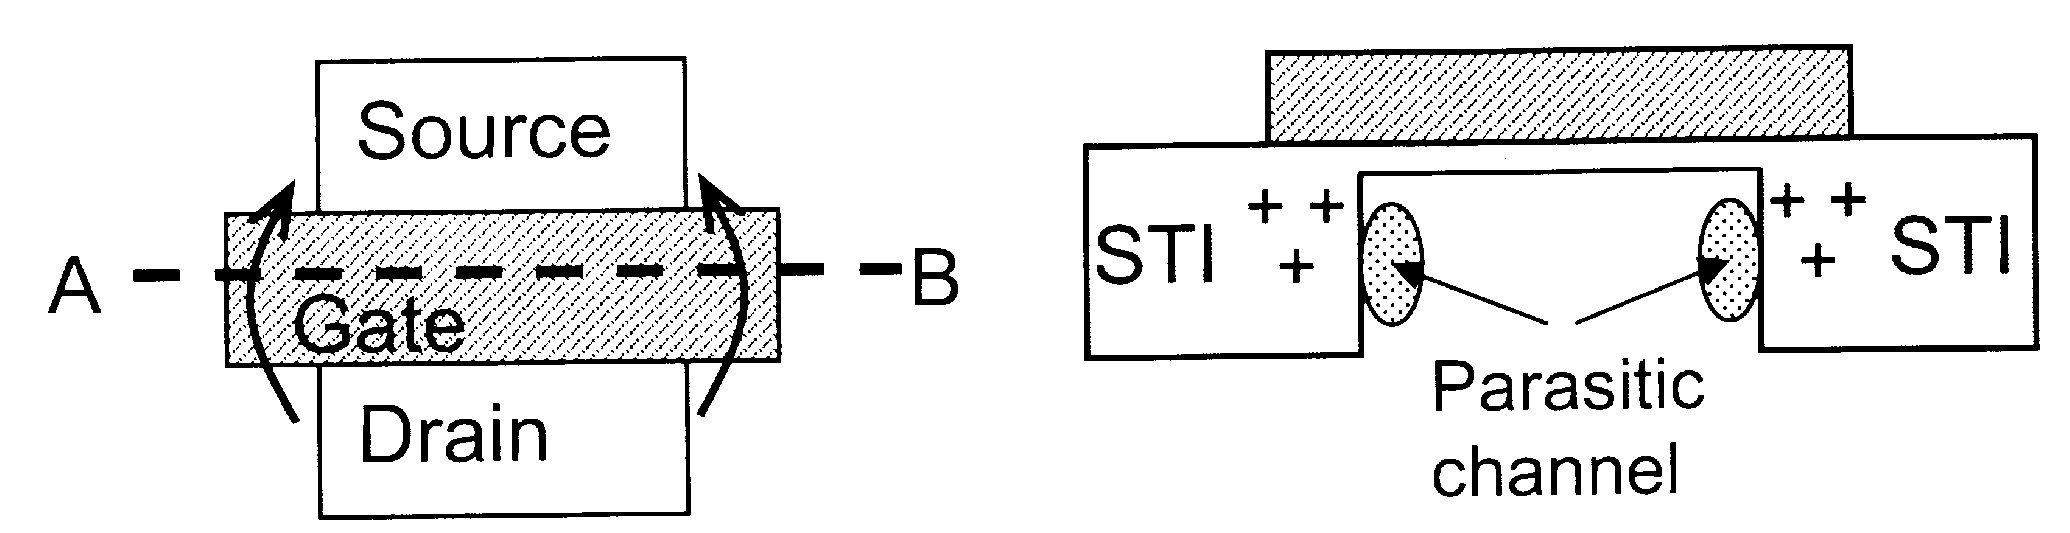
\includegraphics[width=4 in]{RadiationStudies/LeakageCurrent_2.jpg}
\end{center}
\caption{The crosses represent positive charge build up in the shallow trench isolation (STI) oxide, which allow current to pass between the source and the drain when no voltage is applied to the gate\cite{LeakageCurrent}.}
\label{fig:LeakageCurrent}
\end{figure}

Transistors can at least partially recover from these radiation induced damage mechanisms through a process called annealing. This is a complex process that occurs either when trapped charge tunnels out of the oxide or is thermally excited enough to leave the oxide. Once a charge is free from the oxide, it is swept away by oppositely charged voltage contacts of the transistor. 

\section{Experimental Details}

\subsection{Transistor Test Setup}

A 65 nm CMOS Application Specific Integrated Circuit (ASIC) containing individual transistors connected to wire bond pads was built for radiation tolerance testing. Transistors within the ASIC were laid out in groups of similar transistors, for example all N-type metal-oxide-semiconductor (NMOS) transistors with the same channel length (L). Within a group, all transistors share a gate pad and a source/drain pad. The other drain/source of the transistor is connected to its own wire bonding pad, so that each transistor characteristic can be measured individually. The devices tested were P-type metal-oxide-semiconductor (PMOS) and NMOS core transistors operated at 1.2 V and NMOS input/output (I/O) transistors with double thickness gate oxide operated at 2.5 V. Several transistor sizes were included for core PMOS and NMOS transistors: transistors with L $=60$ nm and a channel width (W) between 120 and 1000 nm, one transistor with size W/L $=500/500$ nm, and one with size $5000/5000$ nm. Additionally, triple deep well core NMOS transistors of size 120/60 nm and 5000/60 nm were included with a zero threshold voltage 1500/300 nm transistor and a zero threshold enclosed layout (ELT) 2240/300 nm transistor. The I/O NMOS transistor sizes were W $=280$ nm and L between 400 and 1000 nm, a transistor with size $500/500$ nm, and one with size $5000/5000$ nm. The following different types of I/O NMOS transistors were also included: a triple deep well 800/280 nm transistor, an ELT 2220/280 nm transistor, a zero threshold 3380/1200 nm transistor, and a zero threshold ELT 3450/1200 nm transistor.

The test ASICs were wire bonded into pin grid array (PGA) chip carriers so that they could be irradiated on simple printed circuit boards (PCBs) containing only sockets for the ASICs and connectors for bias voltage. During irradiation PMOS transistors were biased in two different ways: 

\begin{itemize}
\item The drains, sources, and gates were held at 1.2 V and the substrate was grounded. 
\item The gates and substrate were grounded while the drains and sources were held at 1.2 V. 
\end{itemize}
The NMOS core (I/O) transistors were biased with the gates held at 1.2 V (2.5 V) and all other nodes grounded. These are the worst-case bias conditions.

Transistor characteristics were measured by mounting a single chip carrier at a time on a different PCB test board containing switches that allow individual transistors to be measured independently. The test board was connected to two source measurement units (SMUs), one to bias transistor gates and one to measure drain-source currents. Characteristics were made by holding the core (I/O) transistors drain-source voltage at 1.2 V (2.5 V) and the drain-source current was measured as the gate-source voltage was swept from 0 to 1.2 V (2.5 V). 

\subsection{Irradiation Setup}

The irradiation of the test devices was performed at the Gamma Irradiation Facility (GIF) at Sandia National Laboratories.  The GIF uses $\ce{^{60}Co}$ sources to provide controlled doses of ionizing radiation. $\ce{^{60}Co}$ decays by beta decay to an excited state of $\ce{^{60}Ni}$ which then relaxes to the ground state by emitting two gamma rays of energy 1.17 and 1.33 MeV. The $\ce{^{60}Co}$ is held in stainless steel ``source pins'' so that none of the beta electrons escape. 40 source pins are mounted in a straight-line array that is held at the bottom of an 18 foot deep pool of deionized water to provide shielding when not in use and raised out of the water when an irradiation takes place.

The test ASICs were held inside stainless steel thermos bottles positioned approximately two inches from the face of the array of pins. Cooling was provided by vortex tube coolers mounted in holes drilled through the plastic thermos bottle lids. Figure~\ref{fig:Thermos} shows the thermos bottle assembly. To maintain the temperature of the thermos bottles, which were heated by the gamma rays interacting with the walls of the thermos bottles, the compressed air that was input to the vortex tubes was precooled and passed through insulated copper tubes. The temperature within the thermos bottles was measured and recorded by a K-type thermocouple in each thermos bottle. Figure~\ref{fig:Temperature} shows the temperature of two thermos bottles during the irradiations.

\begin{figure}[htbp]
\begin{center}
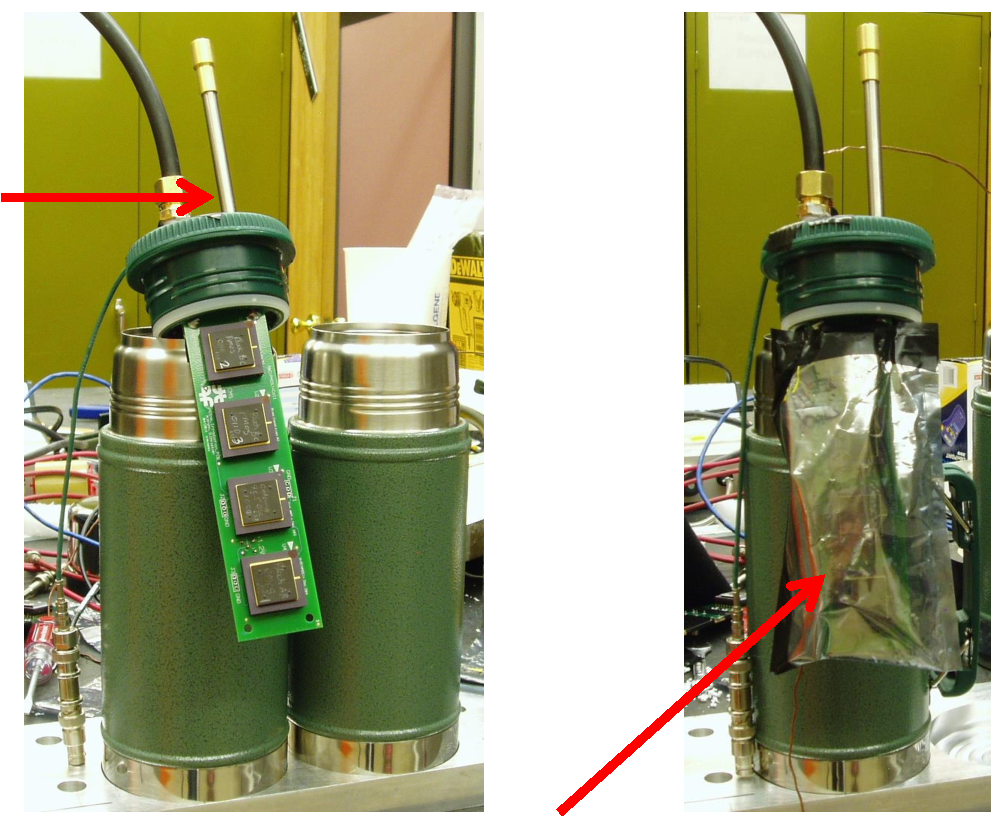
\includegraphics[width=4 in]{RadiationStudies/thermos.pdf}
\end{center}
\caption{Pictures of the thermos bottle, including an irradiation printed circuit board with four chip carriers, before insertion of the irradiation board into the thermos bottle. On the left, the red arrow points to the vortex tube on top of the thermos bottle lid. On the right, the red arrow points to an antistatic bag which wraps the irradiation board and low-voltage cable before irradiation. These bags keep the boards and voltage cables dry during the irradiation.}
\label{fig:Thermos}
\end{figure}

\begin{figure}[htb!]
\begin{center}
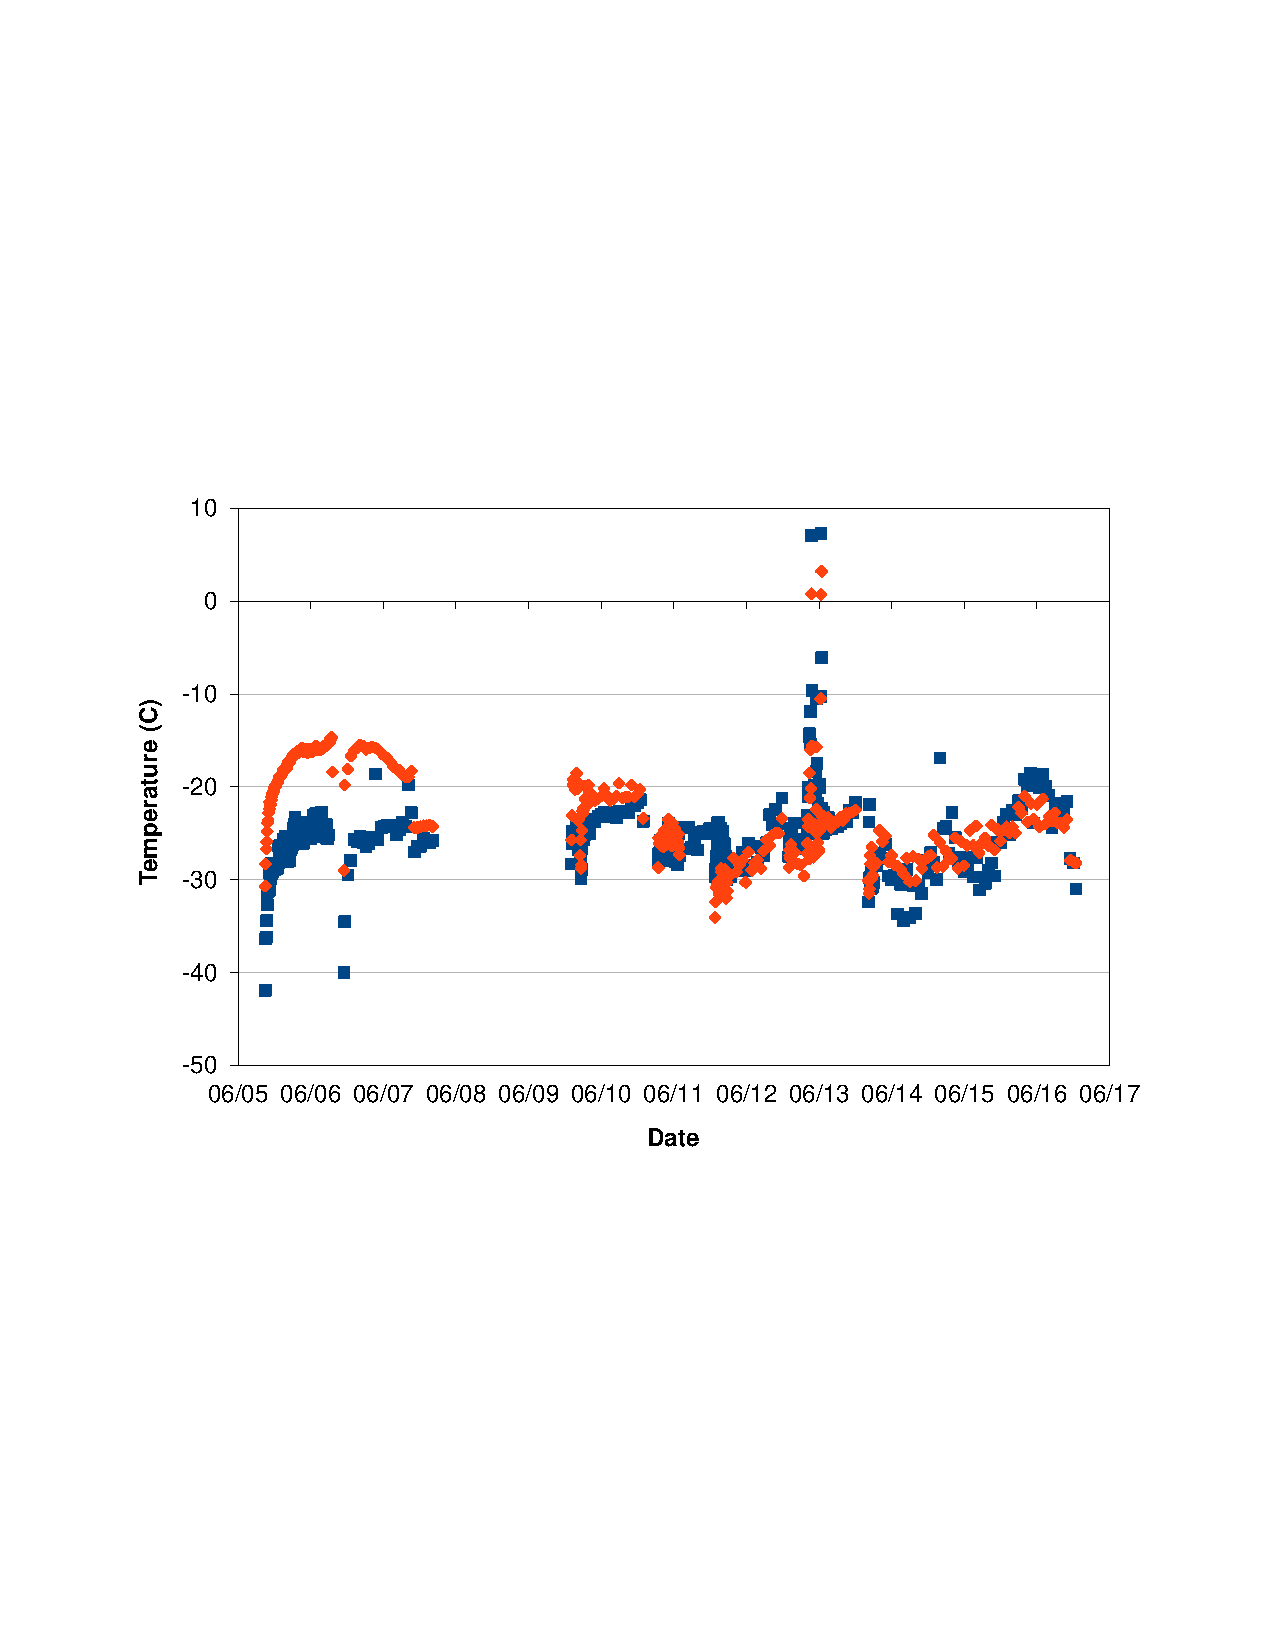
\includegraphics[width=5.5 in]{RadiationStudies/comp_temp.pdf}
\end{center}
\caption{The temperature measured inside the two thermos bottles during the long irradiations. No irradiation was performed on June 8 or 9. The two spikes where the temperature reached about $8^{\circ}\mathrm{C}$ in both thermos bottles for 30 minutes on June 12 occurred because the compressed air unexpectedly turned off.}
\label{fig:Temperature}
\end{figure}

The does rate the test ASICs received was 1425 rad/s and was measured by an ion chamber placed inside of a thermos bottle. The uniformity of the radiation field was checked by irradiating thermoluminescent dosimeters (TLDs) taped to each of the chip carriers on the irradiation PCB. The TLDs also provided a second measurement of the dose rate.

Twelve irradiations were performed over 15 days, as show in Table~\ref{tab:IrradiationSchedule}, and after each irradiation step a single characteristic curve was recorded for each transistor. All measurements were made at room temperature, but when a test ASIC wasn't being irradiated or measured they were stored at $-20^{\circ}\mathrm{C}$ in a freezer. After the full irradiation, devices were kept at room temperature for a week and multiple characteristics were taken to characterize the annealing effects. The transistors were then held in an oven at $100^{\circ}\mathrm{C}$ for one week to simulate an extended annealing period and a final set of measurements was made.

\begin{table}
\begin{center}
\caption{The irradiation schedule, showing the 2 weeks it took to accumulate 1 Grad.}
\begin{tabular}{| p{2cm} | p{2.5cm} | p{2cm} | p{4cm} |}
\hline
Date & Length & Dose(Mrad) & Cumulative Dose(Mrad)\\ \hline
June 2 & 1 hour & 5 & 5\\ \hline
June 3 & 1 hour & 5 & 10 \\ \hline
June 3 & 1 hour 45 mins & 9 & 19 \\ \hline
June 3 & 4 hour 15 mins & 22 & 41 \\ \hline
June 4-5 & 12 hours & 62 & 103 \\ \hline
June 5-6 & 22 hours & 113 & 215 \\ \hline
June 6-7 & 22 hours & 113 & 329 \\ \hline
June 9-10 & 22 hours & 113 & 441 \\ \hline
June 10-11 & 17 hours & 87 & 528 \\ \hline
June 11-12 & 22 hours & 113 & 641 \\ \hline
June 12-13 & 22 hours & 113 & 754 \\ \hline
June 13-16 & 66 hours & 339 & 1093 \\
\hline
\end{tabular}
\label{tab:IrradiationSchedule}
\end{center}
\end{table}


\section{Analysis}

Two quantities were extracted from each transistor characteristic: the maximum drain-source current and the threshold voltage, $V_{th}$. The quadratic extrapolation method was used to determine the threshold voltage~\cite{QuadraticMethod}. As shown in Figure~\ref{fig:QuadraticMethod}, $V_{th}$ is defined to be the voltage at which a line tangent to the curve $\sqrt{|I_{ds}|}$ vs $V_{gs}$ at the point of maximum $\frac{d \sqrt{|I_{ds}|}}{dV_{gs}}$ intercepts the $I_{ds}=0$ axis. The slope of the curve was determined by fitting it with a fifth order polynomial and differentiating the fit function. 

\begin{figure}[htb!]
\begin{center}
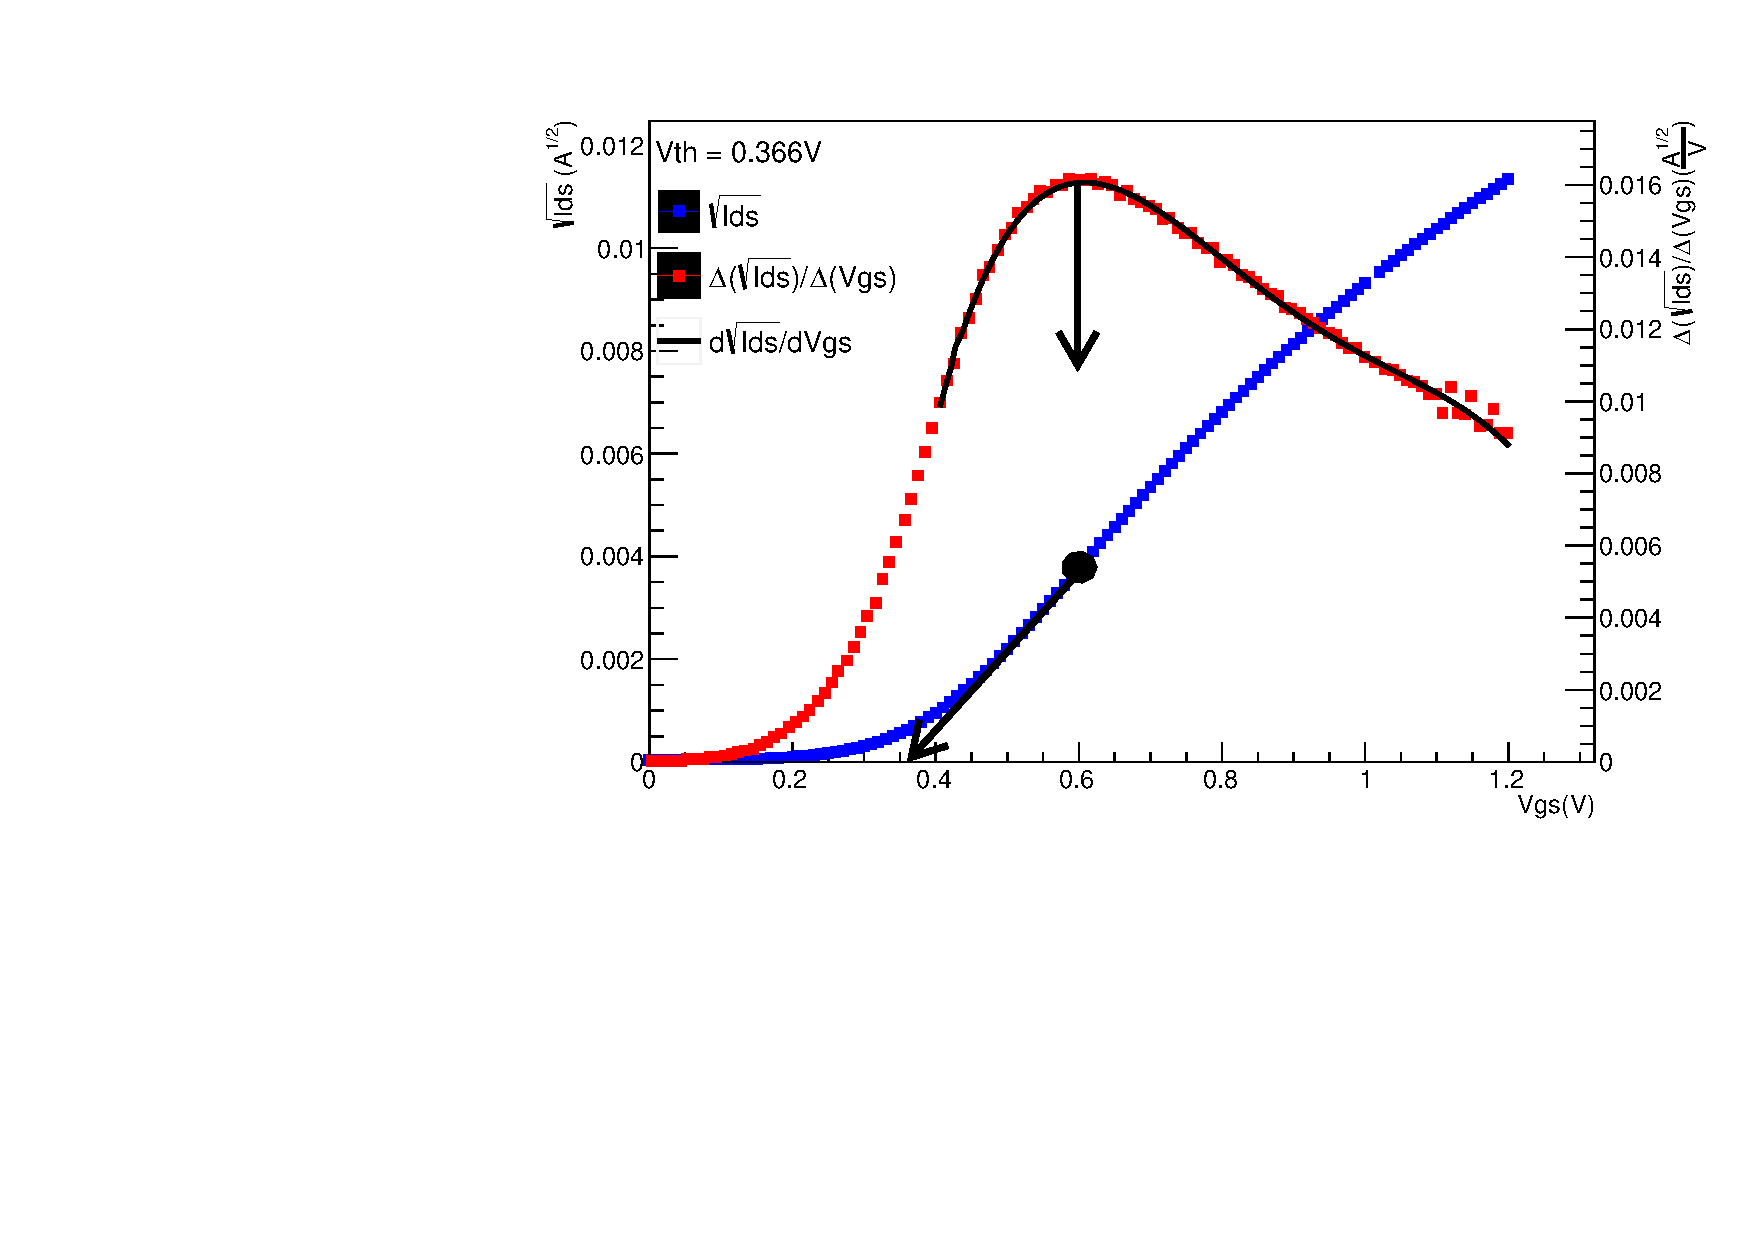
\includegraphics[width=5 in]{RadiationStudies/Quadratic_Method.pdf}
\end{center}
\caption{This figure illustrates the quadratic extrapolation method used to determine the threshold voltage ($V_{th}$) of an NMOS transistor. The blue data points are the transistor characteristic and the red ones are computed using finite differences $\frac{\sqrt{I_{ds}(N+1)}-\sqrt{I_{ds}(N)}}{V_{gs}(N+1)-V_{gs}(N)}$. The black curve is the result of differentiating the fifth order polynomial that was fit to the characteristic. $V_{th}$ is the point on the $I_{ds}=0$ axis where the tangent to the characteristic intersects. For PMOS transistors, $|I_{ds}|$ is used since $I_{ds}$ is negative.}
\label{fig:QuadraticMethod}
\end{figure}

\section{Results}

Figure~\ref{fig:SuperpositionPlots}  illustrates the radiation effects observed in the data.  The most prominent effect is a decrease of the maximum drain-source current of core PMOS transistors.  The fractional decrease is largest for the smallest PMOS transistors and they decreased by more than a factor of two.  No significant difference was observed between the radiation-induced changes of PMOS transistors held at different bias voltages. This is illustrated in Figure~\ref{fig:PMOSBiasConditions}. The maximum drain-source current of core NMOS transistors also decreased, but only by $\sim5-10\%$.  No significant threshold shift was observed for any of the core transistors, but the threshold voltage of NMOS I/O transistors increased by 100 - 200 mV.  

%No error bars are included in the figures because the uncertainty in the SMU measurements is smaller than the symbols used to plot the measurements.

\begin{figure}[htb!]
%	\begin{minipage}[b]{.5\linewidth}
	\begin{subfigure}{.5\linewidth}
	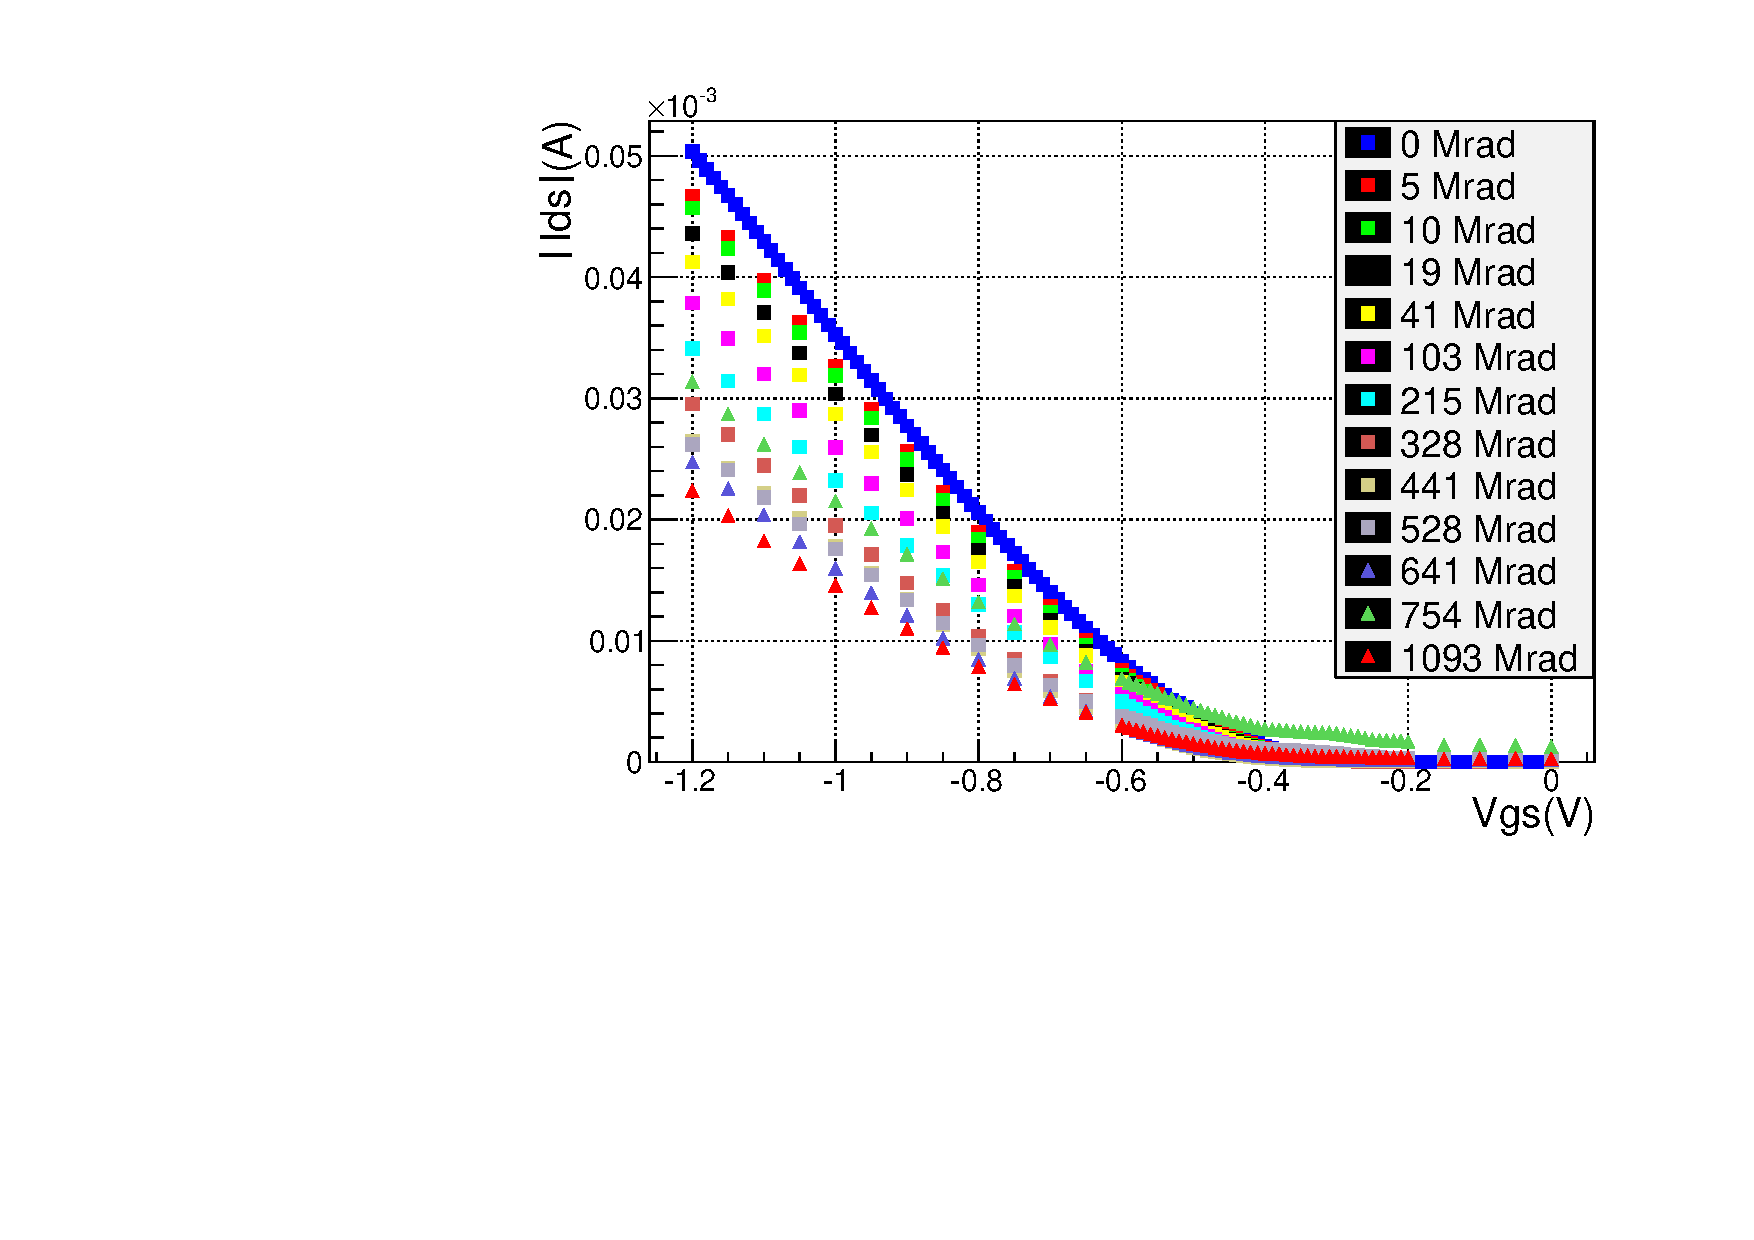
\includegraphics[width=\linewidth]{RadiationStudies/pd012_2_comparison_paper.pdf}
	\end{subfigure}
%	\end{minipage}
%	\begin{minipage}[b]{.5\linewidth}
	\begin{subfigure}{.5\linewidth}
	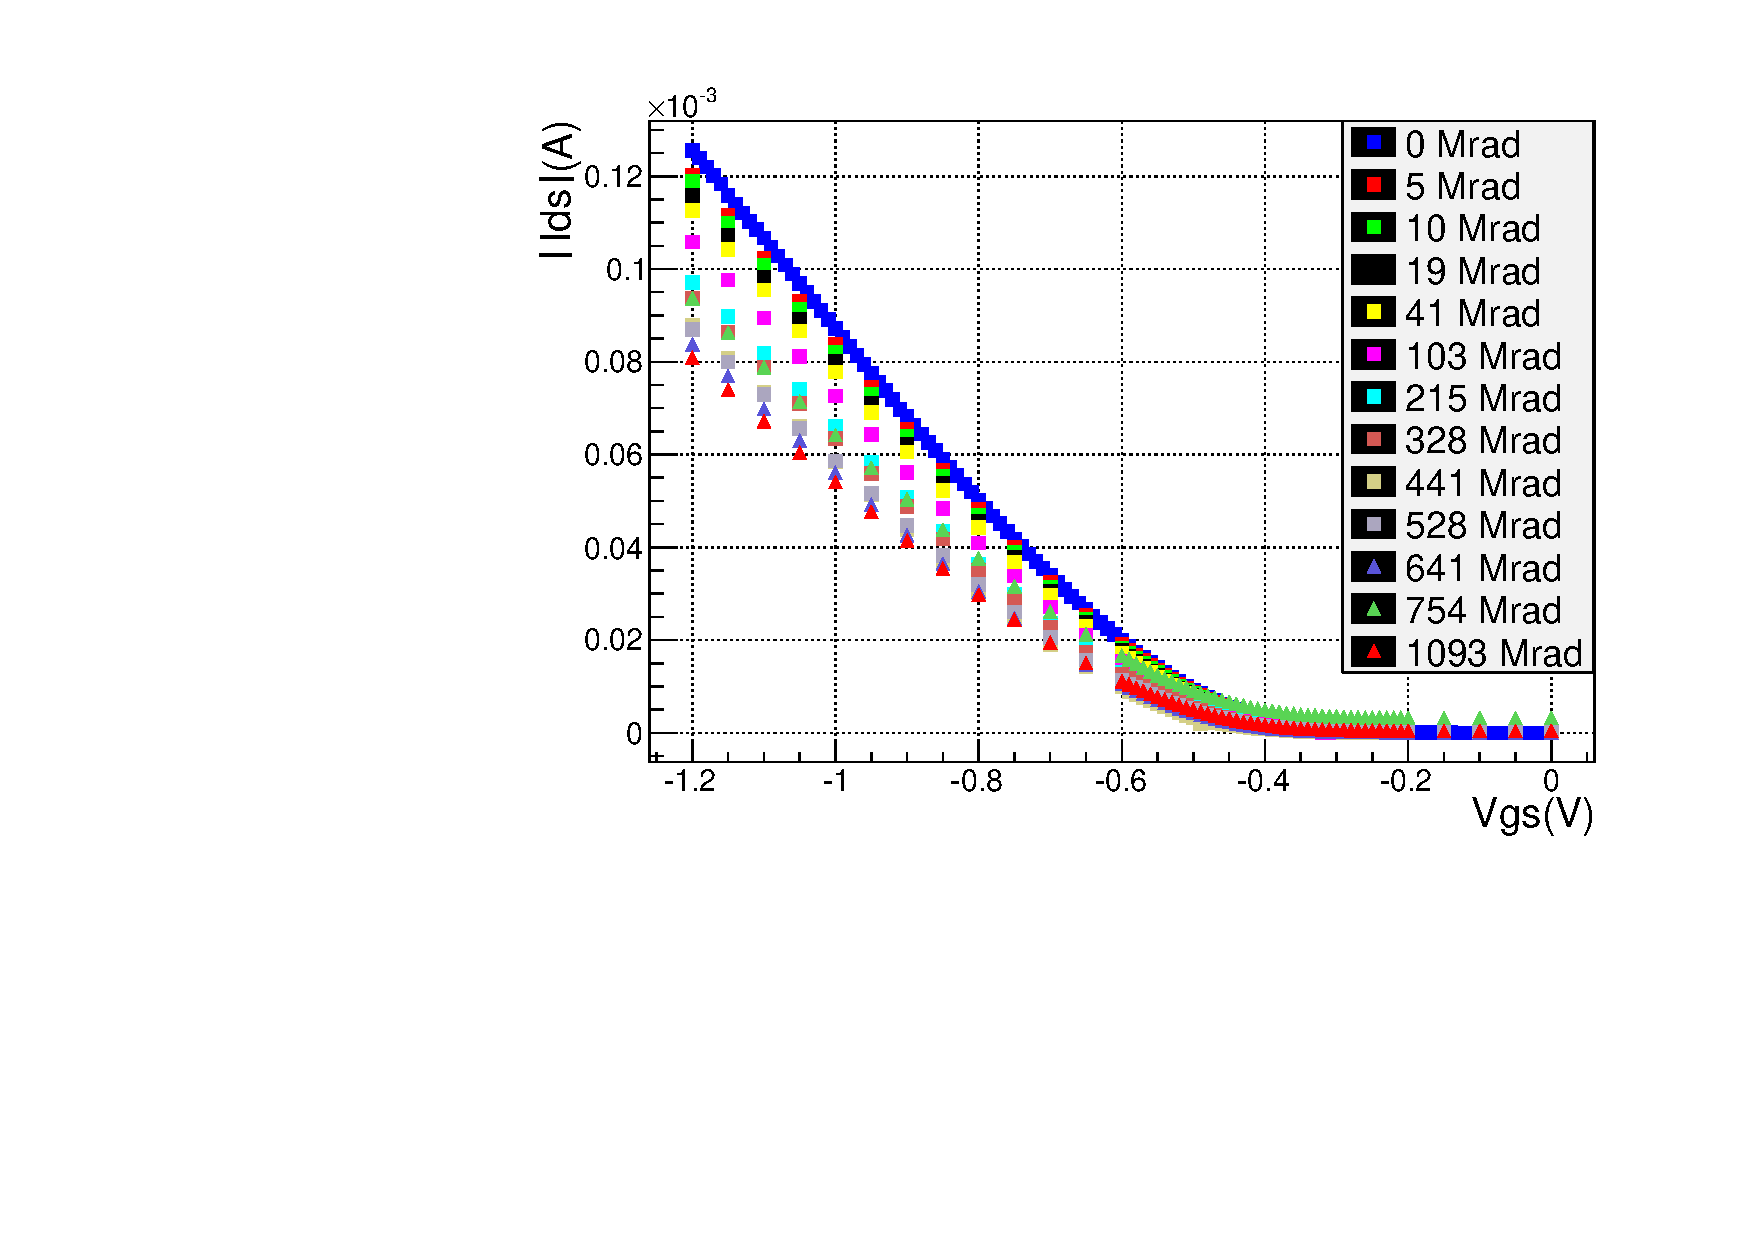
\includegraphics[width=\linewidth]{RadiationStudies/pd036_2_comparison_paper.pdf}
%	\end{minipage}
%	\begin{minipage}[b]{.5\linewidth}
	\end{subfigure}
	\begin{subfigure}{.5\linewidth}
	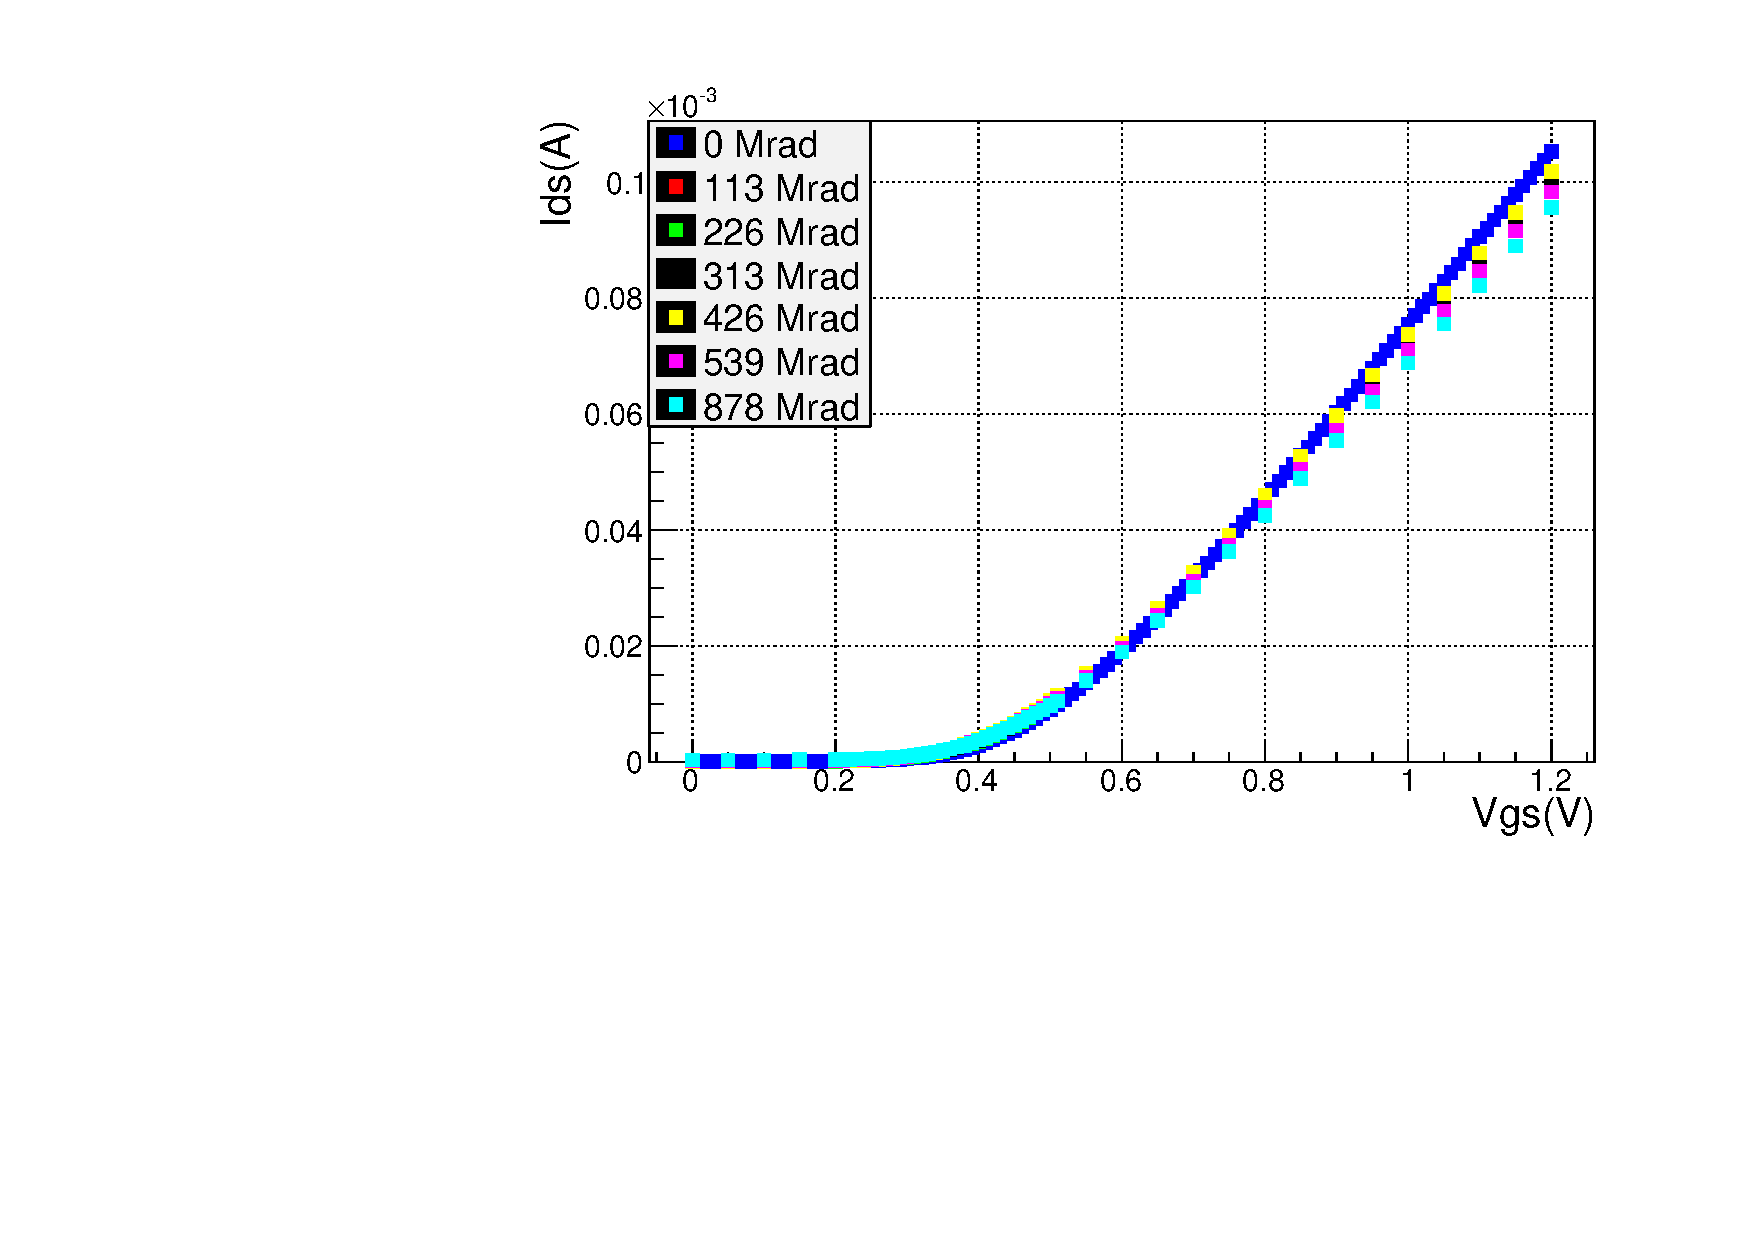
\includegraphics[width=1\linewidth]{RadiationStudies/d024_1_comparison_paper.pdf}
	\end{subfigure}
%	\end{minipage}
	\hfill
%	\begin{minipage}[b]{.5\linewidth}
	\begin{subfigure}{.5\linewidth}
	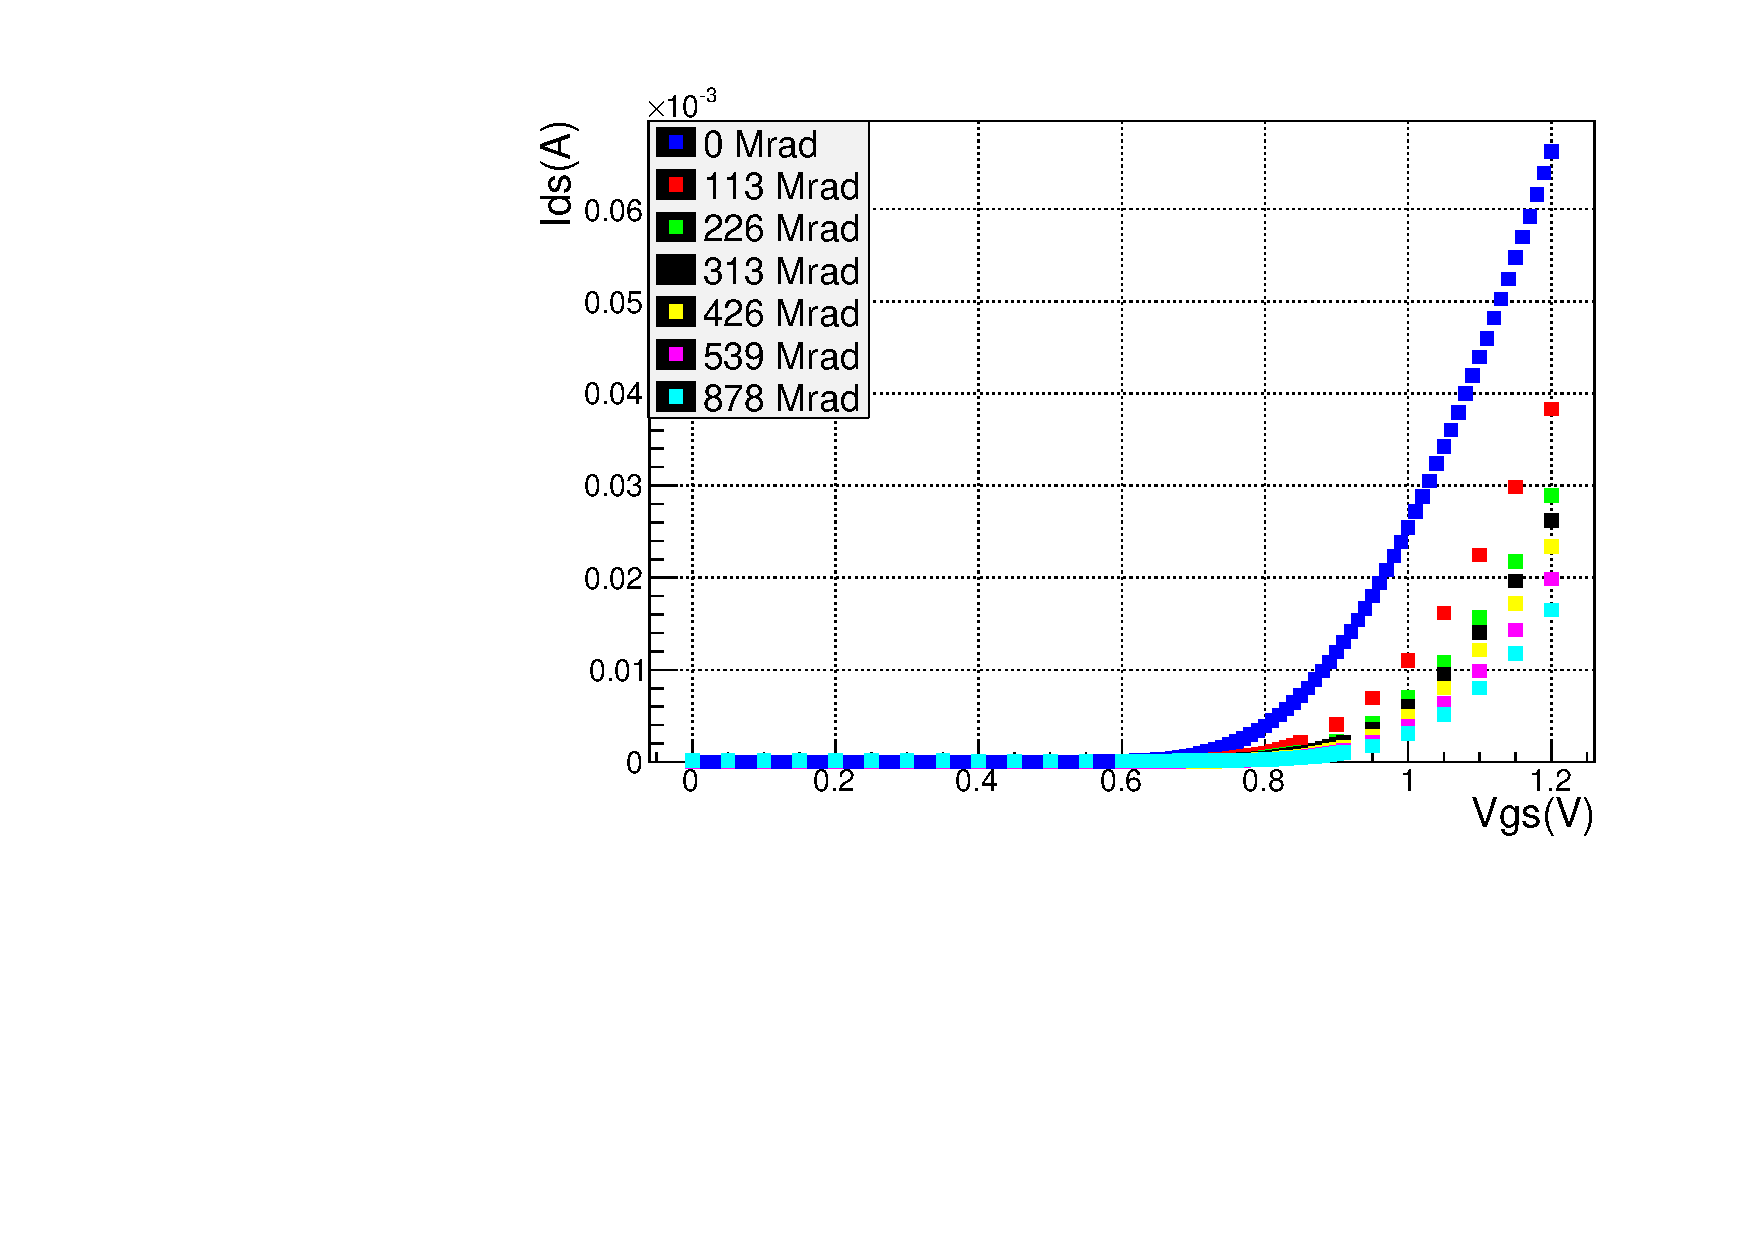
\includegraphics[width=\linewidth]{RadiationStudies/ddg1u_1_comparison_paper.pdf}
	\end{subfigure}
%	\end{minipage}
\caption{Transistor characteristic curves for total dose up to 1.1 Grad of (upper left) a 120/60 core PMOS, (upper right) a 360/60 core PMOS, and for total dose up to 878 Mrad of (lower left) a 240/60 core NMOS, and (lower right) a 1000/280 2.5 V NMOS.}
\label{fig:SuperpositionPlots}
\end{figure}

\begin{figure}[htb!]
	\begin{subfigure}{.5\linewidth}
%\begin{minipage}[b]{0.5\textwidth}
	\centering
	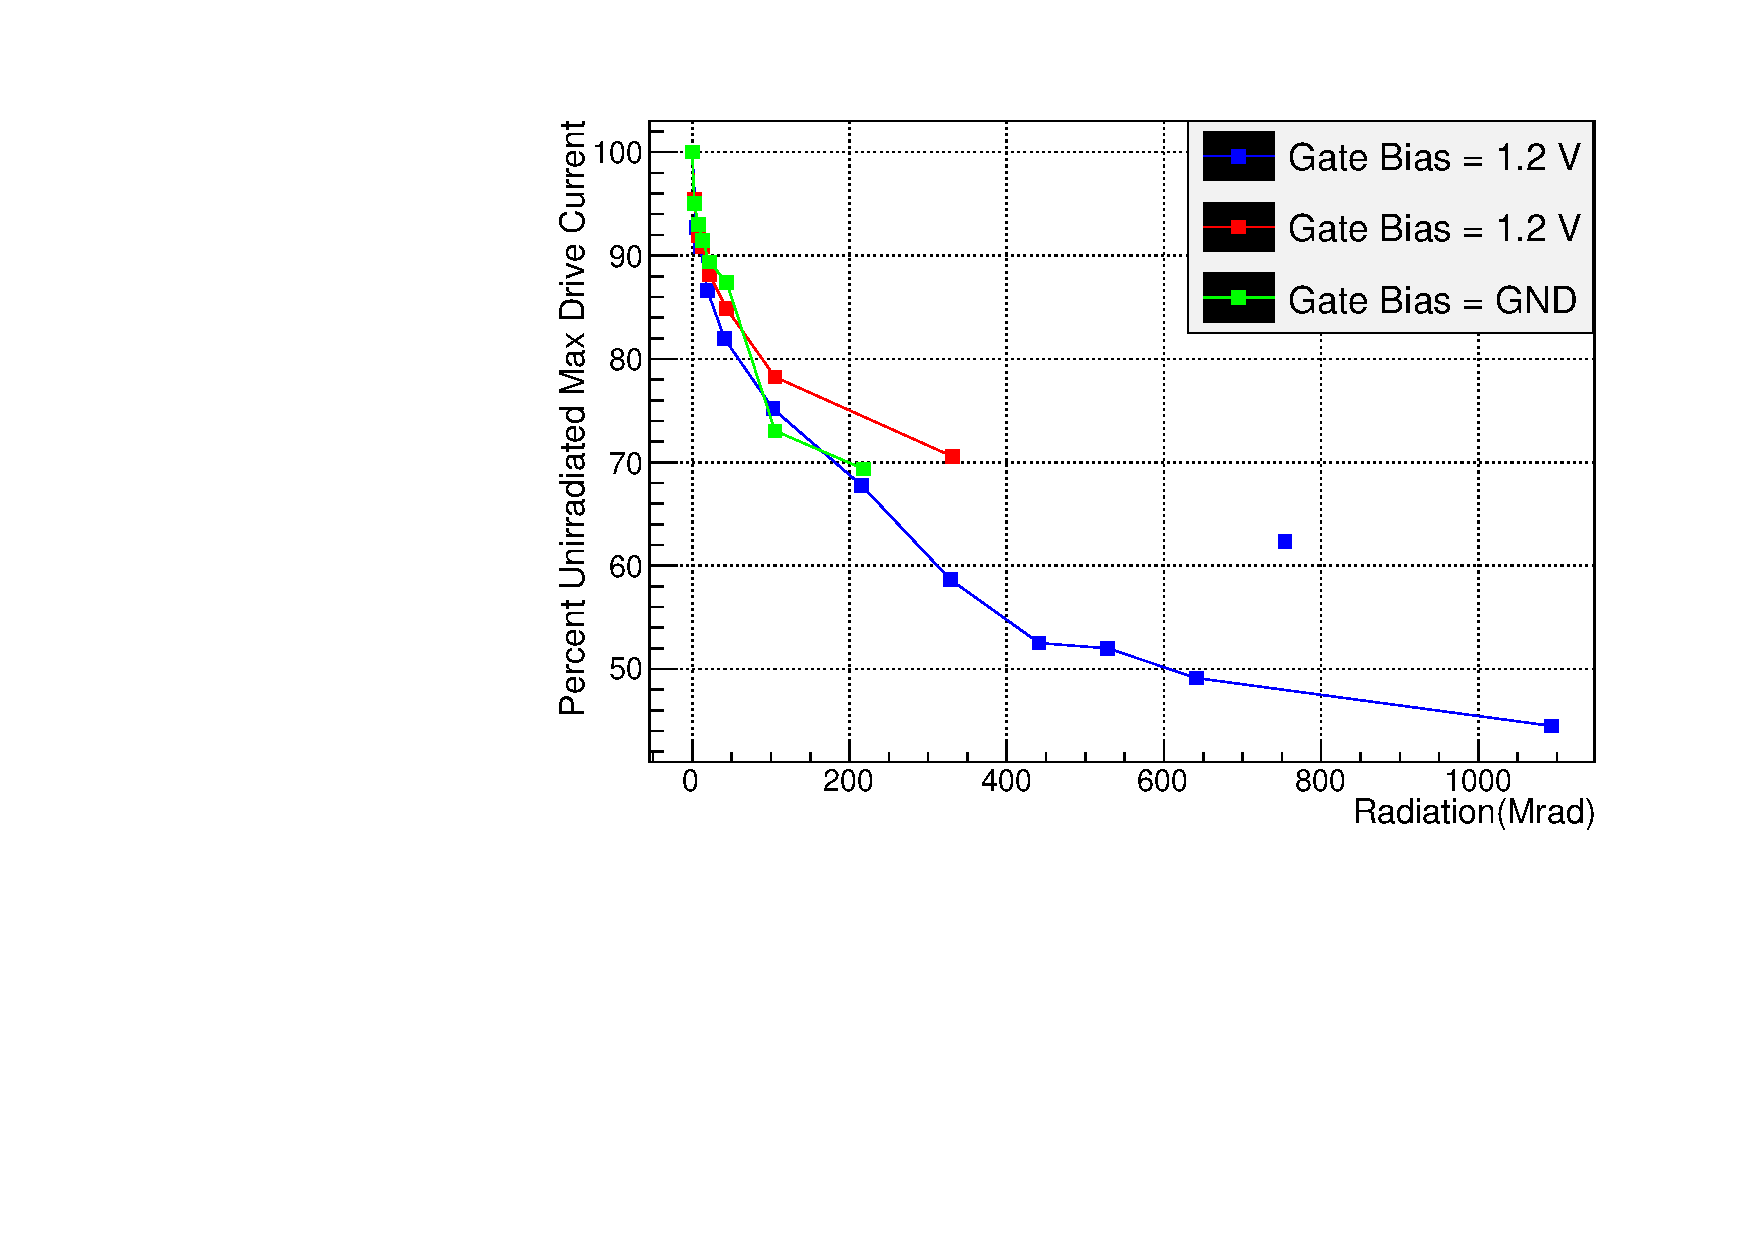
\includegraphics[width=\linewidth]{RadiationStudies/pd012_comparing_bias_conditions_paper.pdf}
	\end{subfigure}
%\end{minipage}
\hspace{0.5cm}
%\begin{minipage}[b]{0.5\textwidth}
	\begin{subfigure}{.5\linewidth}
	\centering
	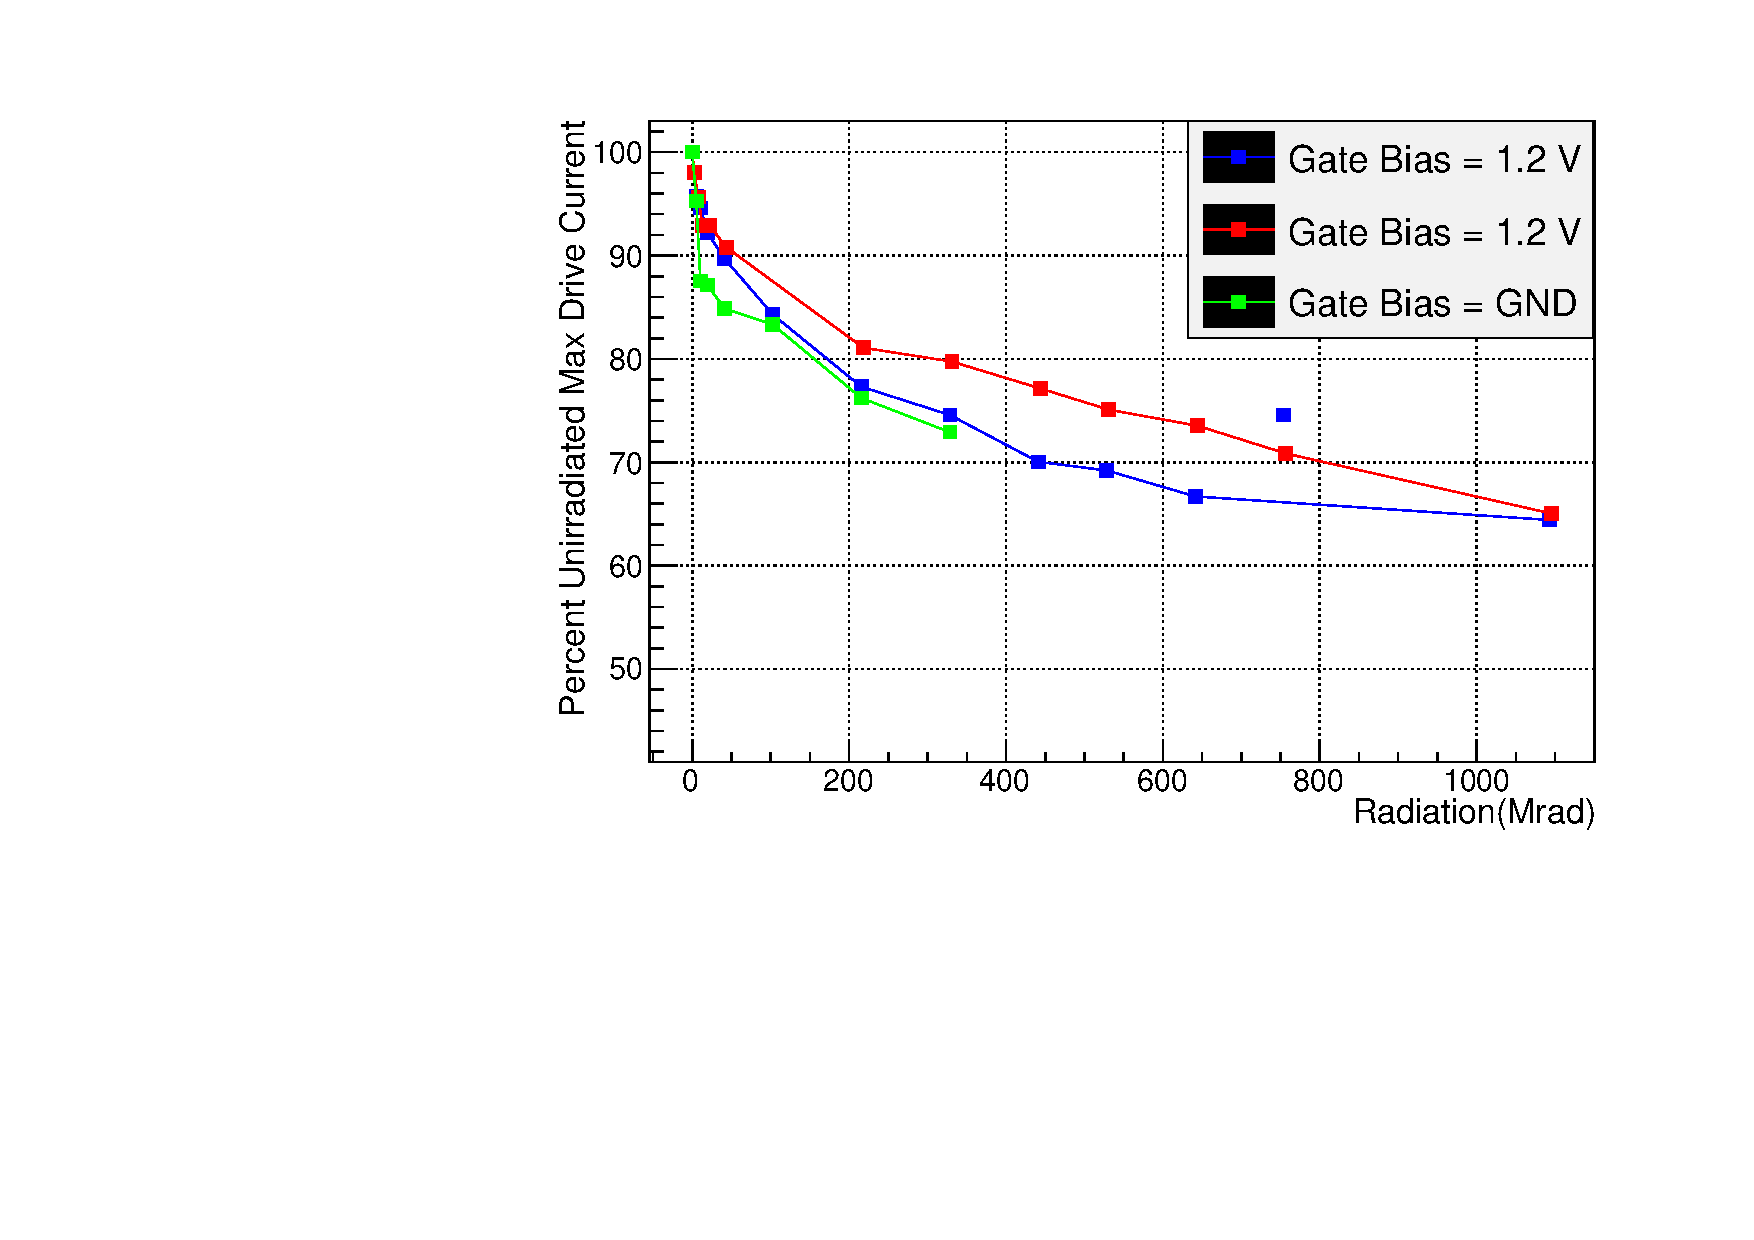
\includegraphics[width=\linewidth]{RadiationStudies/pd036_comparing_bias_conditions_paper.pdf}
	\end{subfigure}
%\end{minipage}
\caption{The change in maximum drain-source current for similar PMOS core transistors irradiated with different gate bias voltages. The graph on the left is for 120/60 transistors and the graph on the right is for 360/60 transistors.  The lines connecting points do not represent a fit, and are included only to make the plots easier to read.  The transistor characteristics measured for transistors in one of the test ASIC packages after 754 Mrad was accumulated were all offset by current not likely to have passed through the transistors (this can be seen in Figure~\ref{fig:SuperpositionPlots}).  Lines are not drawn through these points.  The most likely source of these offsets is leakage current due to moisture caused by condensation on the cold ASIC package.}
\label{fig:PMOSBiasConditions}
\end{figure}

Figure~\ref{fig:AnnealSuperpositionPlots} demonstrates the annealing effects observed in our data. Both the PMOS core transistors and the NMOS I/O transistors recovered significantly during the annealing period. 

\begin{figure}[htb!]
\begin{minipage}[b]{0.5\textwidth}
	\centering
	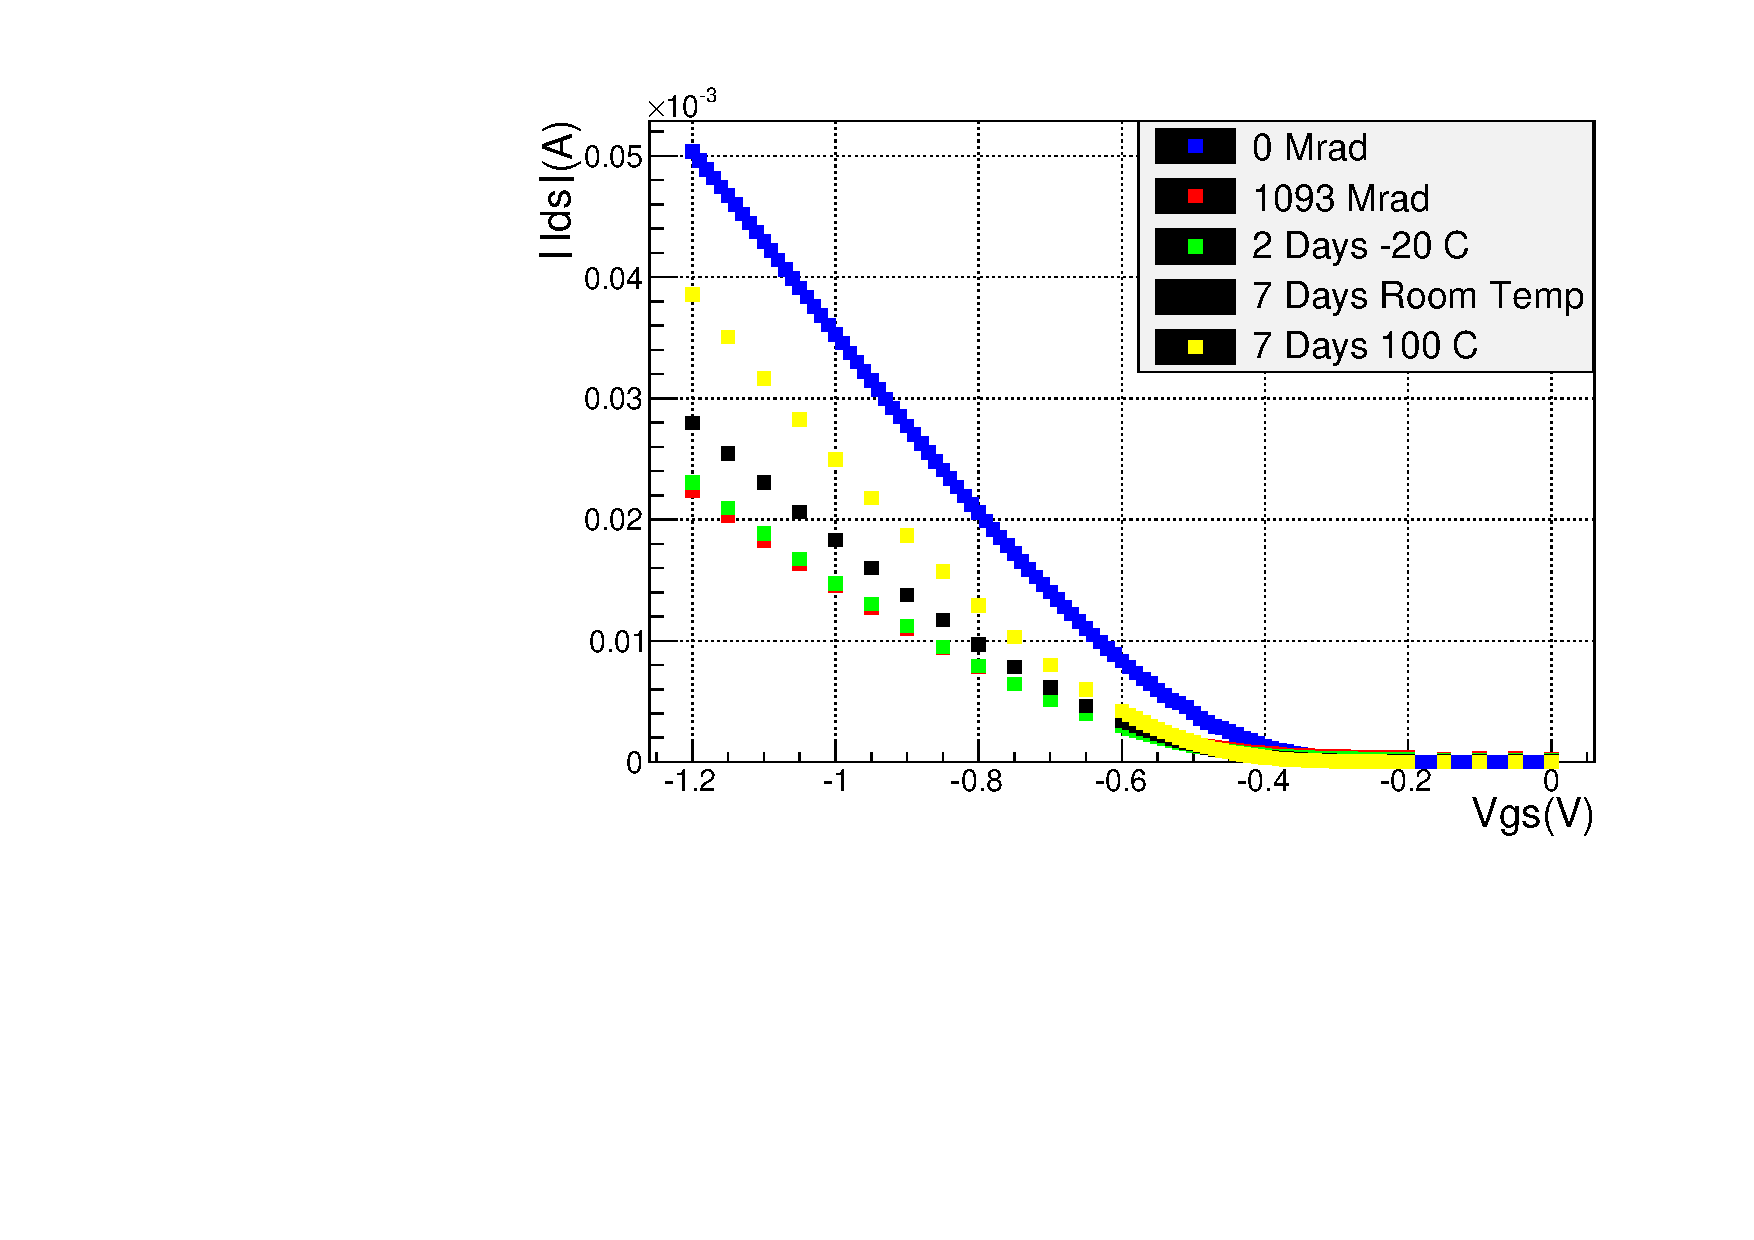
\includegraphics[width=\linewidth]{RadiationStudies/pd012_2_Anneal_comparison_paper.pdf}
\end{minipage}
\hspace{0.5cm}
\begin{minipage}[b]{0.5\textwidth}
	\centering
	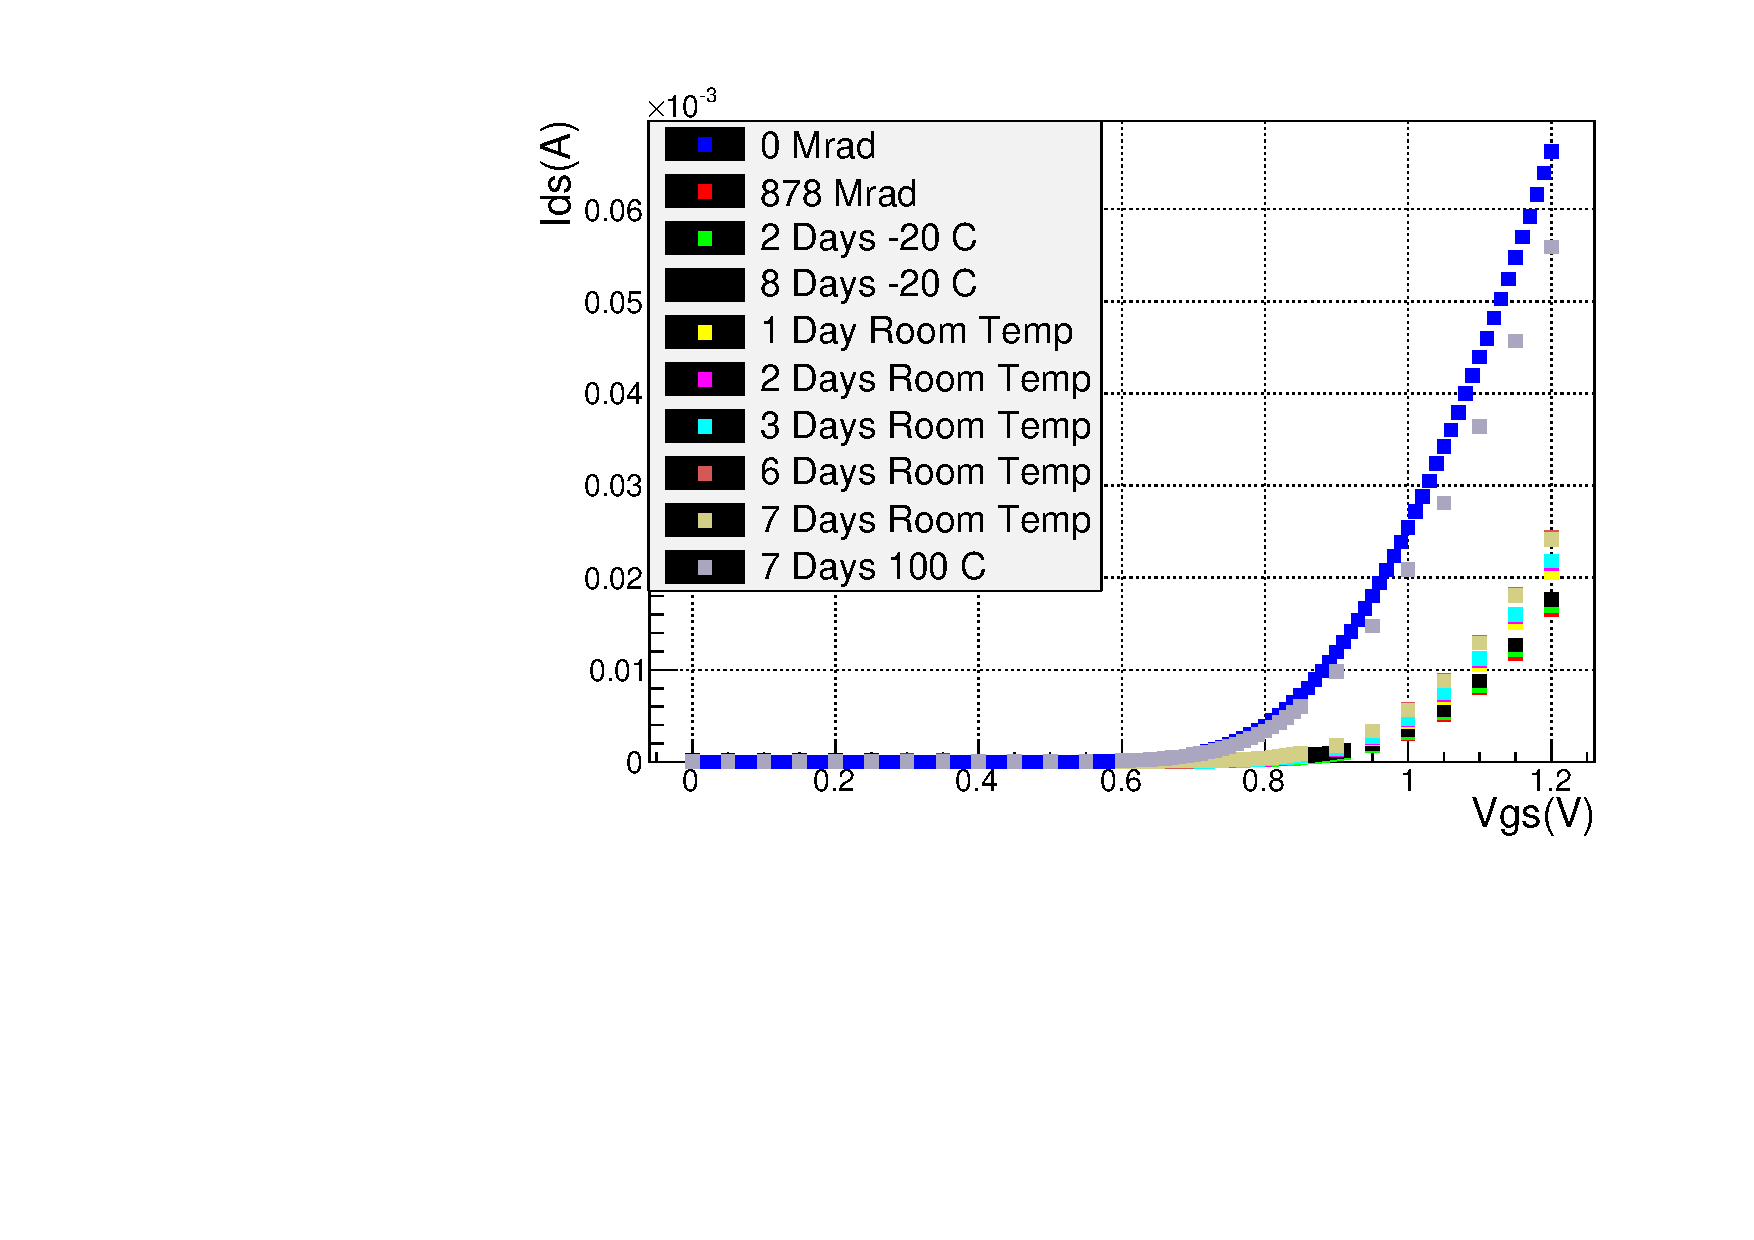
\includegraphics[width=\linewidth]{RadiationStudies/ddg1u_1_Anneal_comparison_paper.pdf}
\end{minipage}
\caption{Transistor chararcteristic curves during the annealing period for (left) a 120/60 core PMOS and (right) a 1000/280 2.5 V NMOS.}
\label{fig:AnnealSuperpositionPlots}
\end{figure}

Figures~\ref{fig:MaxCurDrive_PMOS} and~\ref{fig:MaxCurDrive_NMOS} show the evolution of the maximum drain-source current for a representative selection of PMOS and NMOS core transistors during irradiation and annealing. There were no significant differences in the effect of radiation on the various types of NMOS transistors tested (normal layout, enclosed layout, triple well, and zero $V_{th}$). Figure ~\ref{fig:DGNMOS_Vth} shows the threshold shift of a representative selection of NMOS I/O transistors during irradiation and annealing.

\begin{figure}[htb!]
\begin{minipage}[b]{0.5\textwidth}
	\centering
	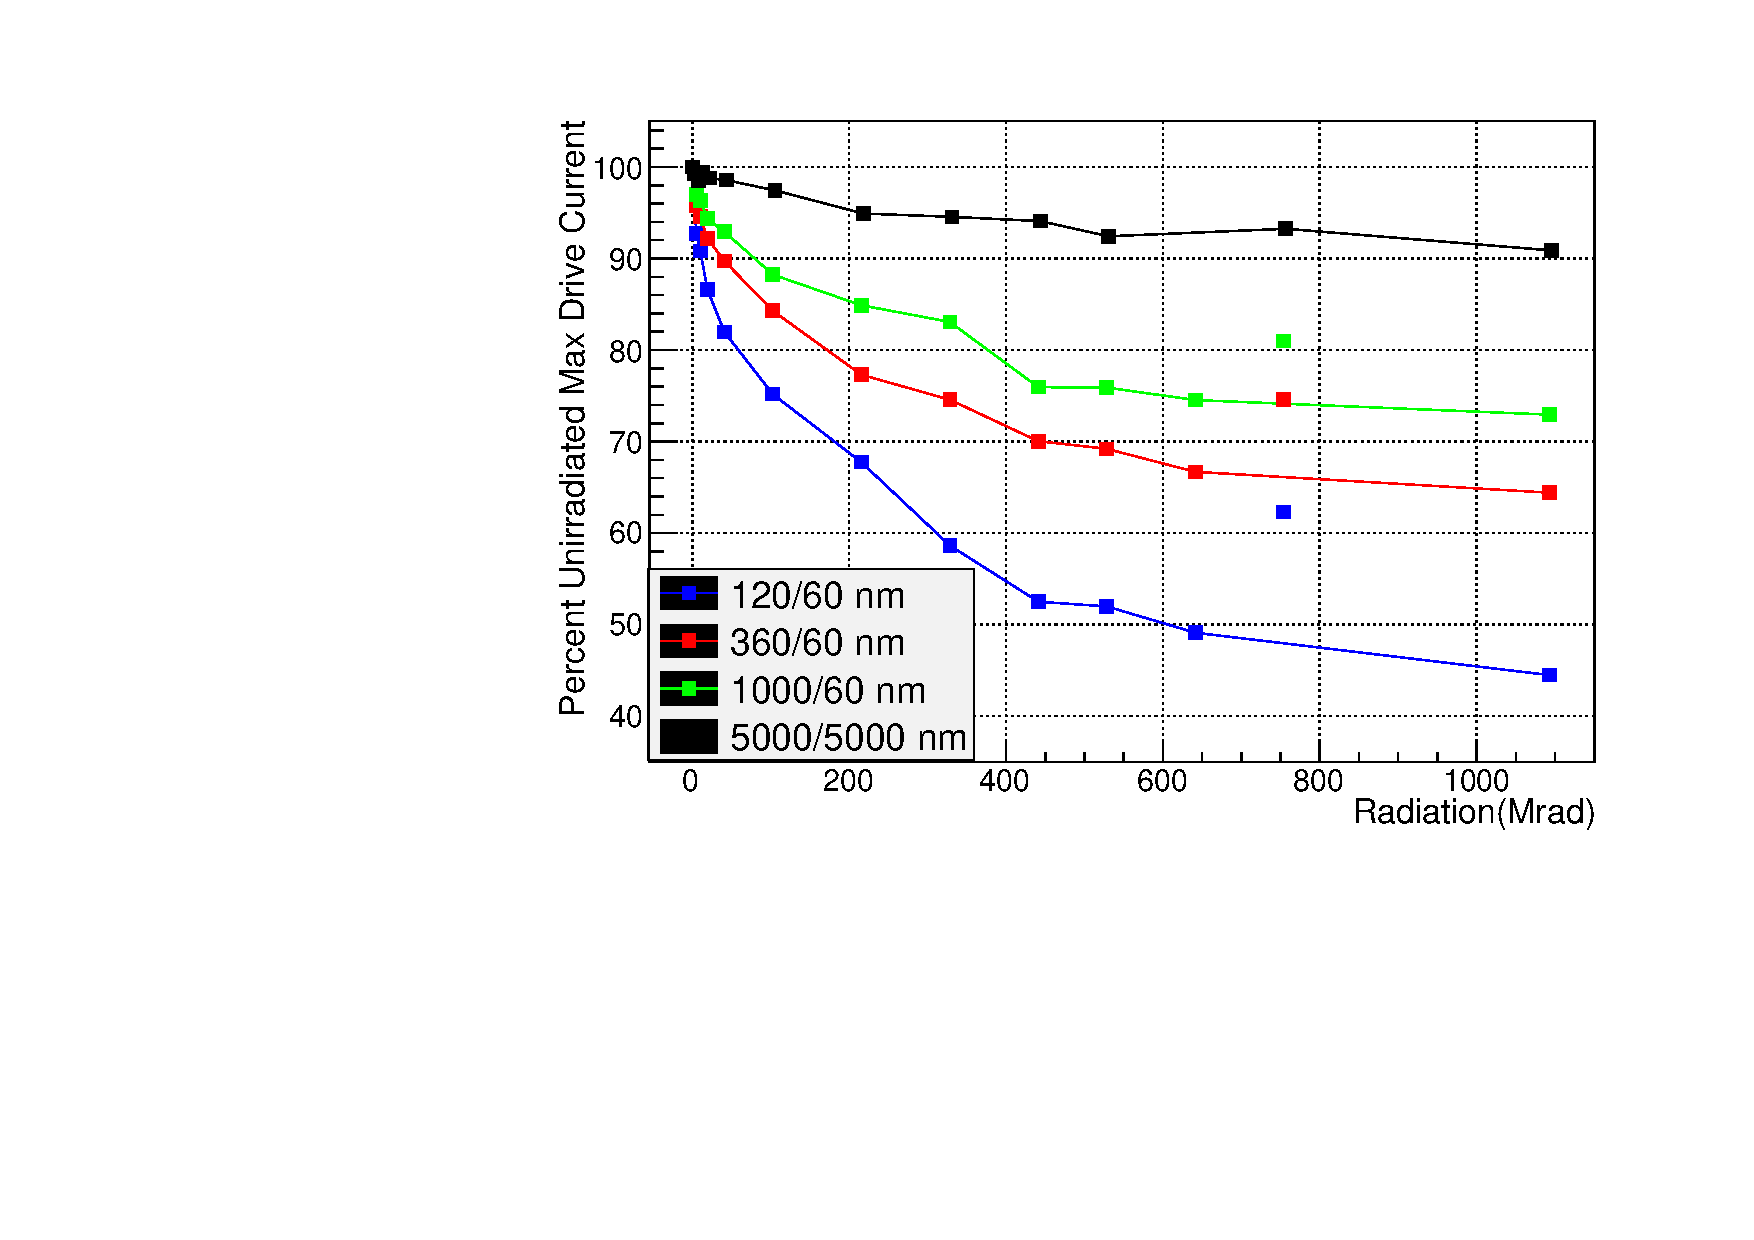
\includegraphics[width=\linewidth]{RadiationStudies/Comparing_MaxCurrentDrive_PMOS_paper.pdf}
\end{minipage}
\hspace{0.5cm}
\begin{minipage}[b]{0.5\textwidth}
	\centering
	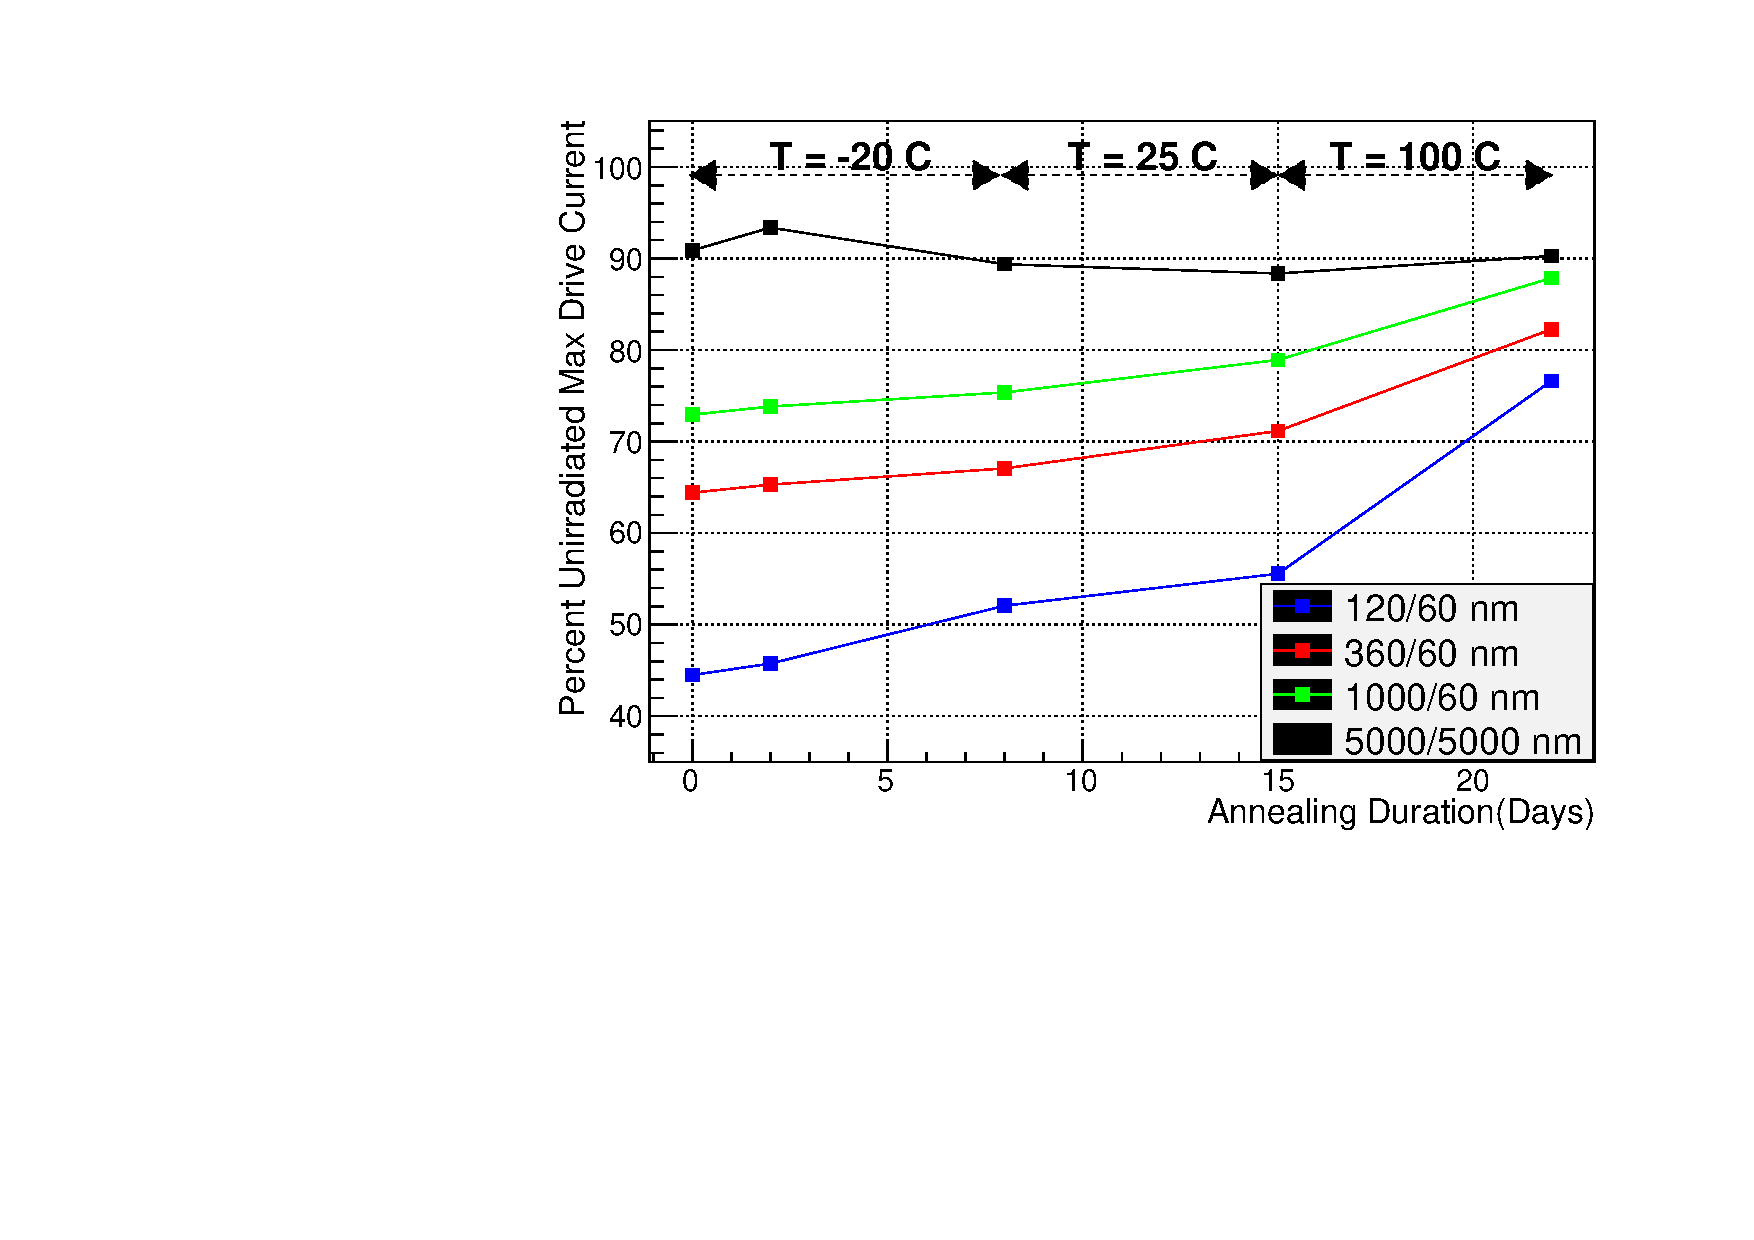
\includegraphics[width=\linewidth]{RadiationStudies/Comparing_MaxCurDrive_Anneal_PMOS_paper.pdf}
\end{minipage}
\caption{The graph on the left shows the loss of maximum drain-source current during irradiation for 4 PMOS core transistors. The graph on the right shows the recovery of maximum drain-source current for the same 4 transistors during and after annealing.
As in Figure~\ref{fig:DGNMOS_Vth}, lines are included to make the plots easier to read.
Once again, lines are not drawn through the points corresponding to measurements made after 754 Mrad of transistors in one of the ASIC packages.}
\label{fig:MaxCurDrive_PMOS}
\end{figure}

\begin{figure}[htb!]
\begin{minipage}[b]{0.5\textwidth}
	\centering
	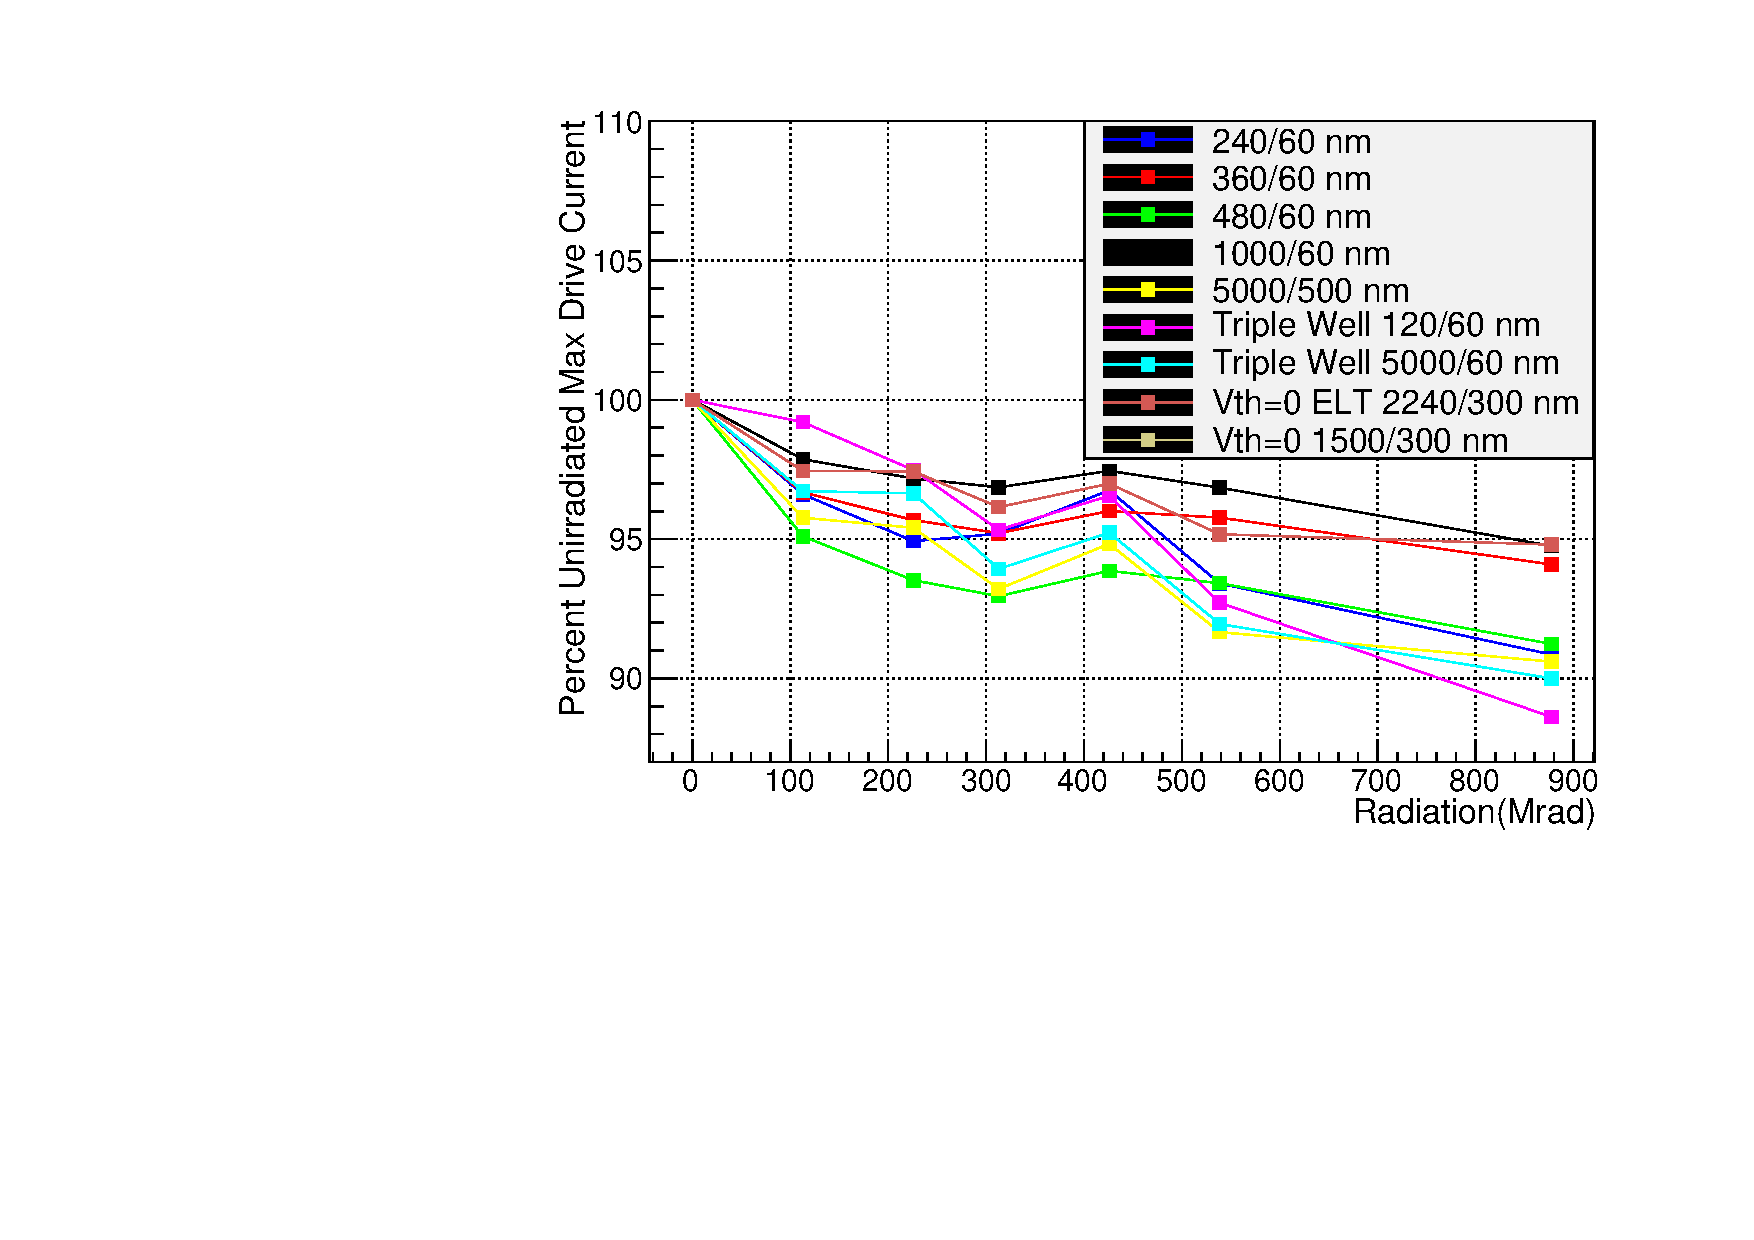
\includegraphics[width=\linewidth]{RadiationStudies/Comparing_MaxCurrentDrive_NMOS_paper.pdf}
\end{minipage}
\hspace{0.5cm}
\begin{minipage}[b]{0.5\textwidth}
	\centering
	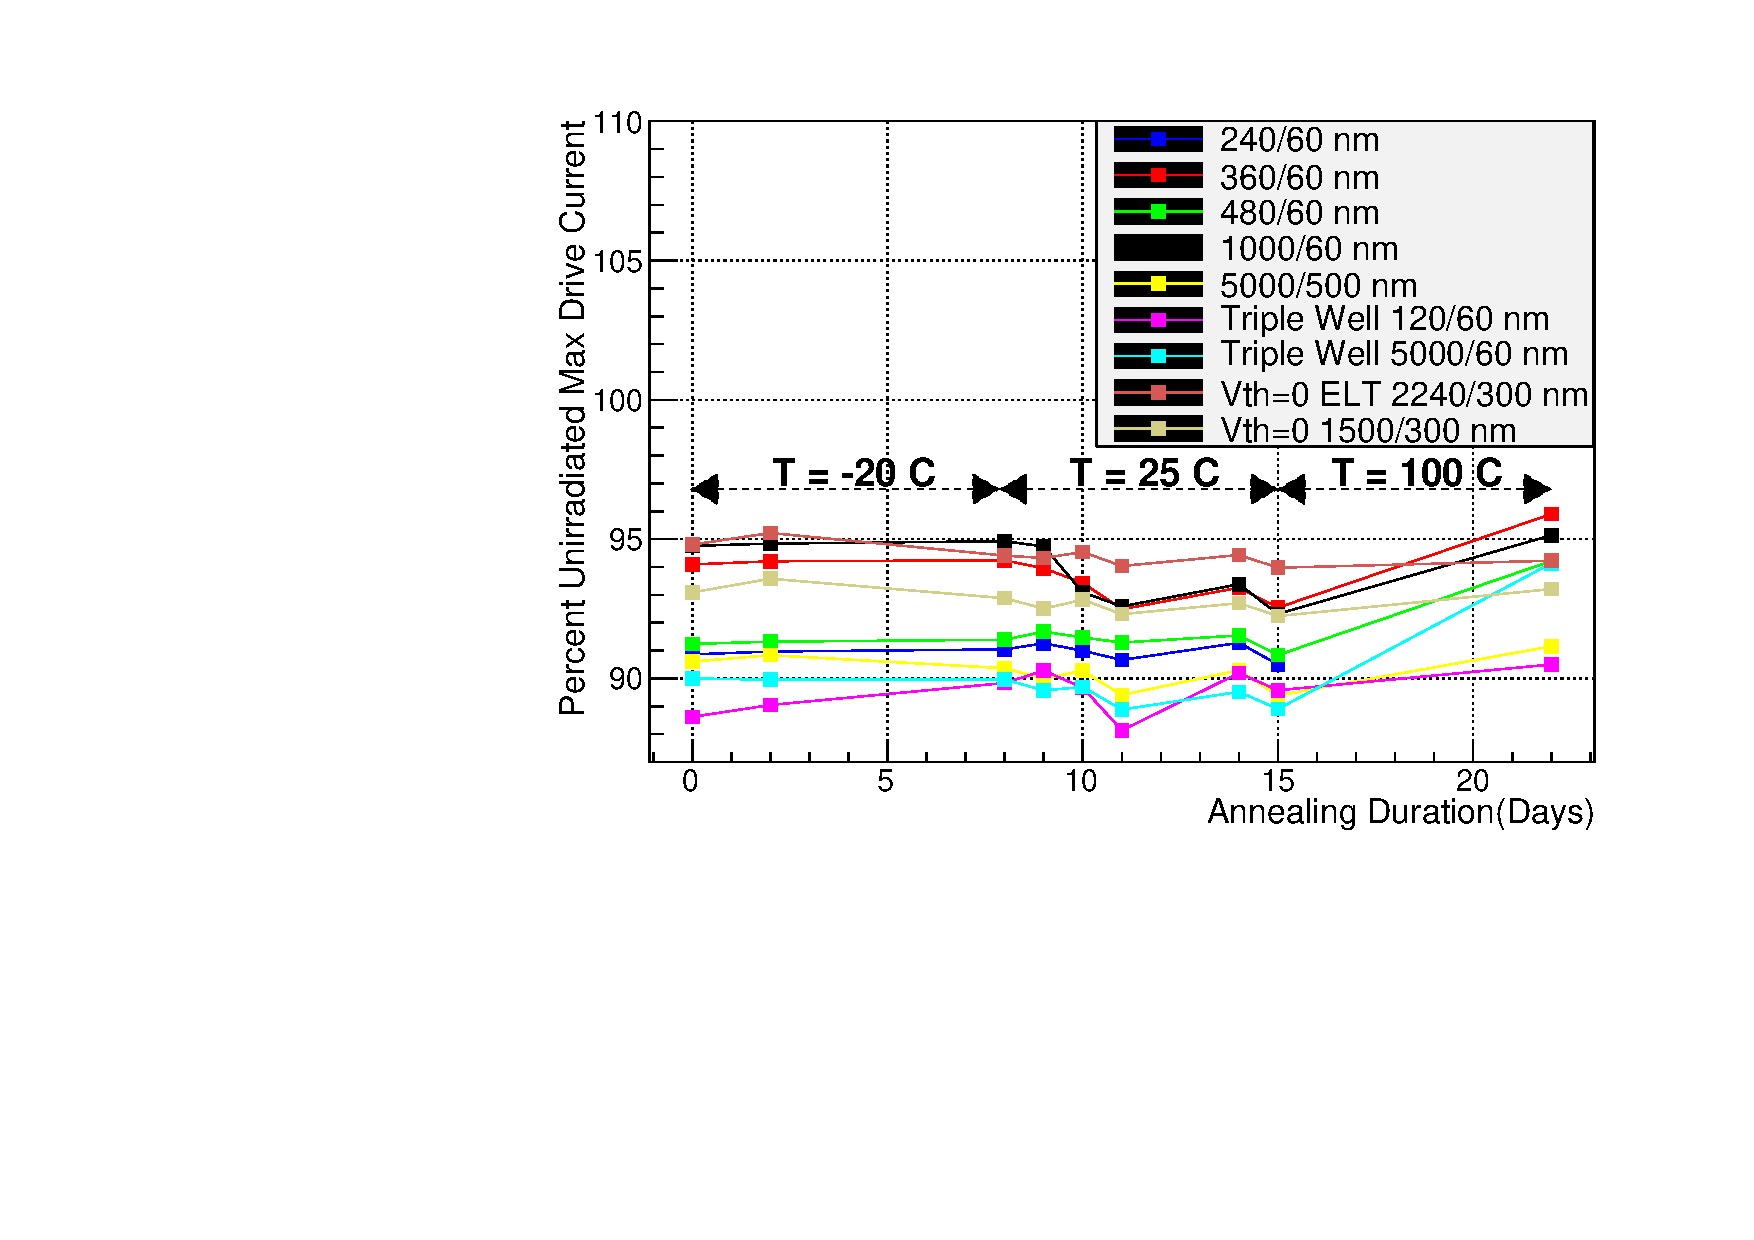
\includegraphics[width=\linewidth]{RadiationStudies/Comparing_MaxCurDrive_Anneal_NMOS_paper.pdf}
\end{minipage}
\caption{The graph on the left shows the loss in maximum drain-source current after each irradiation step for 9 NMOS core transistors. The graph on the right shows the change in maximum drain-source current for the same 9 transistors during and after annealing.}
\label{fig:MaxCurDrive_NMOS}
\end{figure}

\begin{figure}[htb!]
\begin{minipage}[b]{0.5\textwidth}
	\centering
	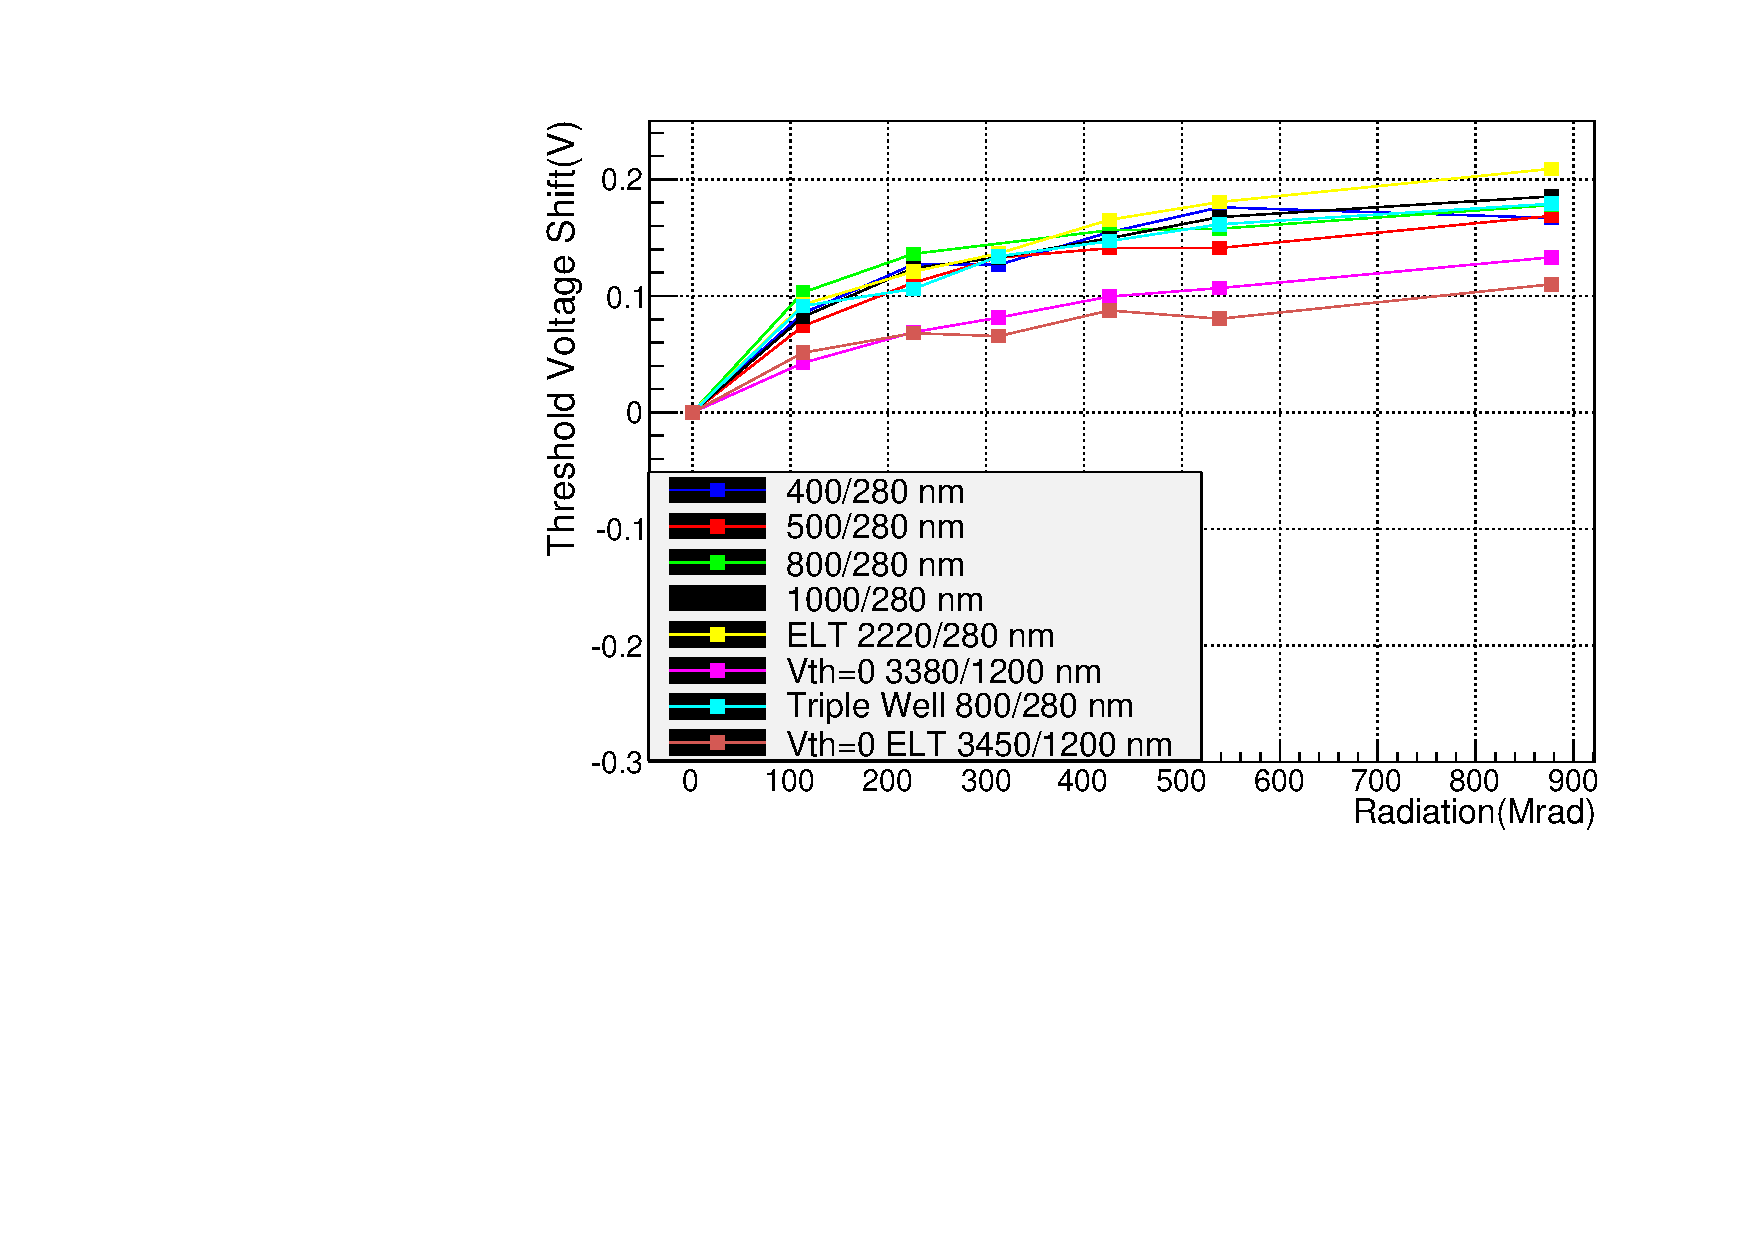
\includegraphics[width=\linewidth]{RadiationStudies/Comparing_ThreshVolt_DGNMOS_paper.pdf}
\end{minipage}
\hspace{0.5cm}
\begin{minipage}[b]{0.5\textwidth}
	\centering
	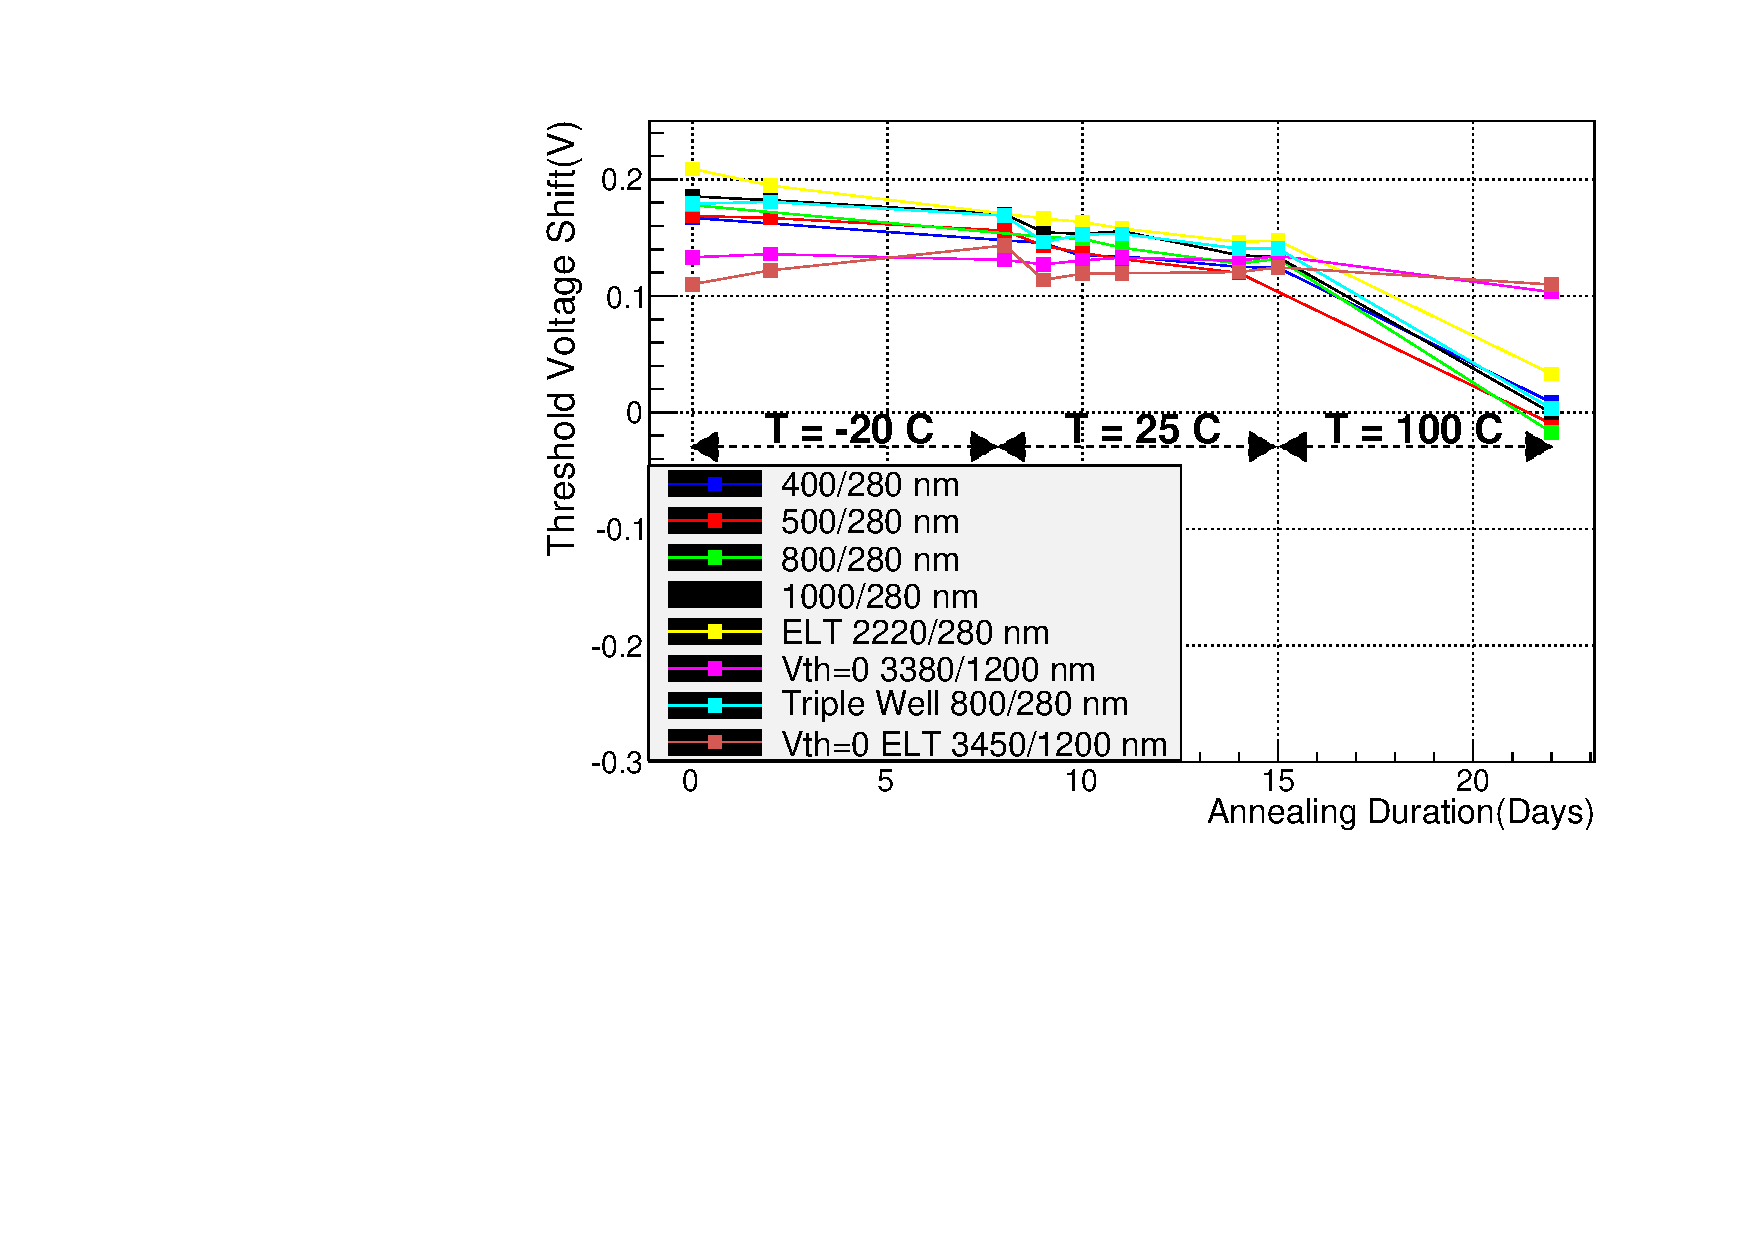
\includegraphics[width=\linewidth]{RadiationStudies/Comparing_ThreshVolt_Anneal_DGNMOS_paper.pdf}
\end{minipage}
\caption{The shift in threshold voltage for 8 NMOS I/O transistors irradiated to 878 MRad is shown in the graph on the left, while the graph on the right shows $V_{th}$ for the same 8 transistors during and after annealing.  No significant annealing was observed for the two zero $V_{th}$ I/O transistors.}
\label{fig:DGNMOS_Vth}
\end{figure}

\section{Summary}

The irradiation of 65 nm CMOS transistors held at $-20^{\circ}\mathrm{C}$ was motivated by the need to simulate the actual operating conditions of the HL-LHC CMS pixel detector. The results show the same pattern of effects that had been observed at room temperature irradiations except the damage observed was less severe, rather than more severe. This could be due to holes and electrons traveling slower through the oxide at lower temperatures and thus, recombining more often\cite{RINCE}.

These studies show that 65 nm CMOS transistors are a viable option for electronics within the HL-LHC CMS pixel detector.

















